\documentclass{article}

\usepackage[margin=1in]{geometry}
\usepackage{amsmath}  
\usepackage{graphicx} 
\usepackage{float}
\usepackage{booktabs}
\usepackage{caption}
\usepackage{hyperref}

\usepackage{xcolor}
\hypersetup{
    colorlinks,
    linkcolor={red!50!black},
    citecolor={blue!50!black},
    urlcolor={blue!70!black}
}

\newcommand{\multisum}{\ensuremath{\mathop{\sum_{i=0}^n \sum_{i=j}^n \sum_{k=0}^{n} \sum_{l=0}^n}_{i+j+k+l \le n} }}

\begin{document}
    \title{Damage distributions for deterministic and stochastic rotations}
    \author{By @cherryjesus}
    \date{}
    \maketitle

    \section{Introduction}\label{sec:intro}

    Many jobs have deterministic rotations in the sense that skills, abilities, and buffs are performed at specific times and neither the rotation nor the damage distribution varies when the rotation is repeated. In contrast, some jobs have stochastic rotations because the effects and number of usages for certain skills, abilities, and/or buffs depend on chance. Each time a stochastic rotation is repeated, it will differ from the previously executed rotation. Stochastic rotations can further be categorized into two major cases: (i) skills/buffs where the total number of hits is randomly distributed and (ii) buffs where the effects are randomly distributed. Specific examples of the first case include the number of Bloodletter hits a Bard lands or how many Lord of Crowns an Astrologian draws will be random each time the rotation is performed. For the second case, examples include buffs like Astrologian's Astrodyne depending on the number of unique seals or whether an individual receives an Astrologian's Card. 
    
    The random nature of stochastic rotations is important because they impart variability to the distribution of damage dealt in addition to variability already present from hit types and damage rolls. Here, two methods for computing damage distributions of deterministic rotations will be developed. The methods used to compute deterministic damage distributions will then be extended to average over both cases of stochastic rotations.\footnote{The examples here will typically be for the simplest possible cases to illustrate the methods. There will be footnotes for how more complicated cases can be handled, when applicable.}

    \section{Deterministic rotations: (asymptotically) exact damage distributions}\label{sec:deterministic}

    We begin by developing two ways of computing the distribution of damage dealt for a deterministic rotation. The first method is exact where the other method is asymptotically exact as the total number of hits approaches infinity, but is also cheaper to evaluate. While the damage distribution could be approximated via sampling, this introduces sampling error and directly calculating probability distributions will often be computationally cheaper. 
    
    For this section, we briefly review how damage dealt is calculated and the notation will follow {``Variability in damage calculations''}. The total number hits for a given ability/skill is denoted as $n_h$. The probability for each hit type is 
    \begin{equation}\label{eqn:probability}
        \textbf{p} = [1 - p_C - p_D + p_{CD}, p_C - p_C p_D, p_D  - p_C p_D, p_C p_D]
    \end{equation}
    where $p_C$ and $p_D$ are the hit type rates from Critical Hit and Direct Hit Rate stats, respectively. The order of the elements is the probability of landing a normal hit (NH), a critical hit given a critical-direct hit does not occur (CH), a direct hit given a critical-direct hit does not occur (DH), and a critical-direct hit (CDH).\footnote{The order of hit types for vectors will always be normal, critical, direct, and critical-direct.} The damage dealt for a given hit type is 

    \begin{equation}\label{eqn:d3}
        D_3 = \lfloor \lfloor \lfloor D_2 \lambda_C \rfloor / 1000 \rfloor \lambda_D \rfloor / 100 \rfloor
    \end{equation}

    where $D_2$ is the damage dealt after accounting for potency, attack power, determination, etc. and $\lambda_C$ and $\lambda_D$ are the damage modifiers for a critical hit and direct hit, respectively.\footnote{
        This is the same $D_2$ from \href{https://docs.google.com/document/d/1OpfKYmf31FpES3IHOrl3H8phU4Np8FChH4B4lP1ZE08/}{``{How to be a Math Wizard - Third Edition}''}
    } The additional damage dealt by these hit types are

    \begin{equation}
        \begin{split}
            \lambda_C &= 1000 + f_{CH}[CH] \\
            \lambda_D &= 100 + 25[DH]
        \end{split}
    \end{equation}
    where $f_C$ is the damage modifier for a critical hit and the quantity $[\cdot]$ represents an Iverson bracket for whether a critical hit or direct hit occurred. After the hit type is determined, an additional $\pm 5\%$ of damage is rolled from a uniform distribution, $D$
    \begin{equation}\label{eqn:final-dmg}
        % D = \mathcal{U}\{ \lfloor \lfloor \lfloor 0.95 D_3 \rfloor B_1 \rfloor B_2 \rfloor, 
        % \lfloor \lfloor \lfloor 1.05 D_3 \rfloor B_1 \rfloor B_2 \rfloor \}
        D = \left\lfloor \mathcal{U}\{ \lfloor 0.95 D_3 \rfloor, \lfloor 1.05 D_3  \rfloor \} \prod_{i}B_i \right\rfloor.
    \end{equation}
    The support for hit type $i$ is given by

    \begin{equation}\label{eqn:supp}
        \textrm{supp}(D_i) = \{\lfloor d  \prod_j B_j \rfloor \}
        % _{d = \lfloor 0.95 D_{3,i} \rfloor}^{\lfloor 1.05 D_{3,i} \rfloor} 
        \:\: d \in \{\lfloor 0.95 D_{3,i} \rfloor, \lfloor 1.05 D_{3,i} \rfloor \},   
    \end{equation}
    and $D_i$ is uniformly distributed,
    \begin{equation}\label{eqn:single-hit-pmf}
        P(D_i) = \left|\textrm{supp}(D_i) \right|^{-1},
    \end{equation}
    where $\left|D_i \right|^{-1}$ is the number of elements in the sequence defined by eqn. \ref{eqn:single-hit-pmf}. The distribution of damage dealt for landing a single hit is given by the mixture distribution

    \begin{equation}
        P(D; n_h = 1) = \sum_{i \in [\textrm{NH}, \textrm{CH}, \textrm{DH}, \textrm{CDH}]} p_i P(D_i) 
    \end{equation}
    where $P(D_i)$ is the damage distribution for hit type $i$ after the damage roll and $p_i$ is the probability of landing hit type $i$ (eqn. \ref{eqn:probability}). An example of the (unweighted) component distributions and the resulting mixture distribution is shown in Figure \ref{fig:1-hit-mixture}.\footnote{The damage distributions will have some gaps in the support because of the floor operator. These gaps are not shown here for clarity, but are present in calculations.}
    \begin{figure}[H]
        \centering
        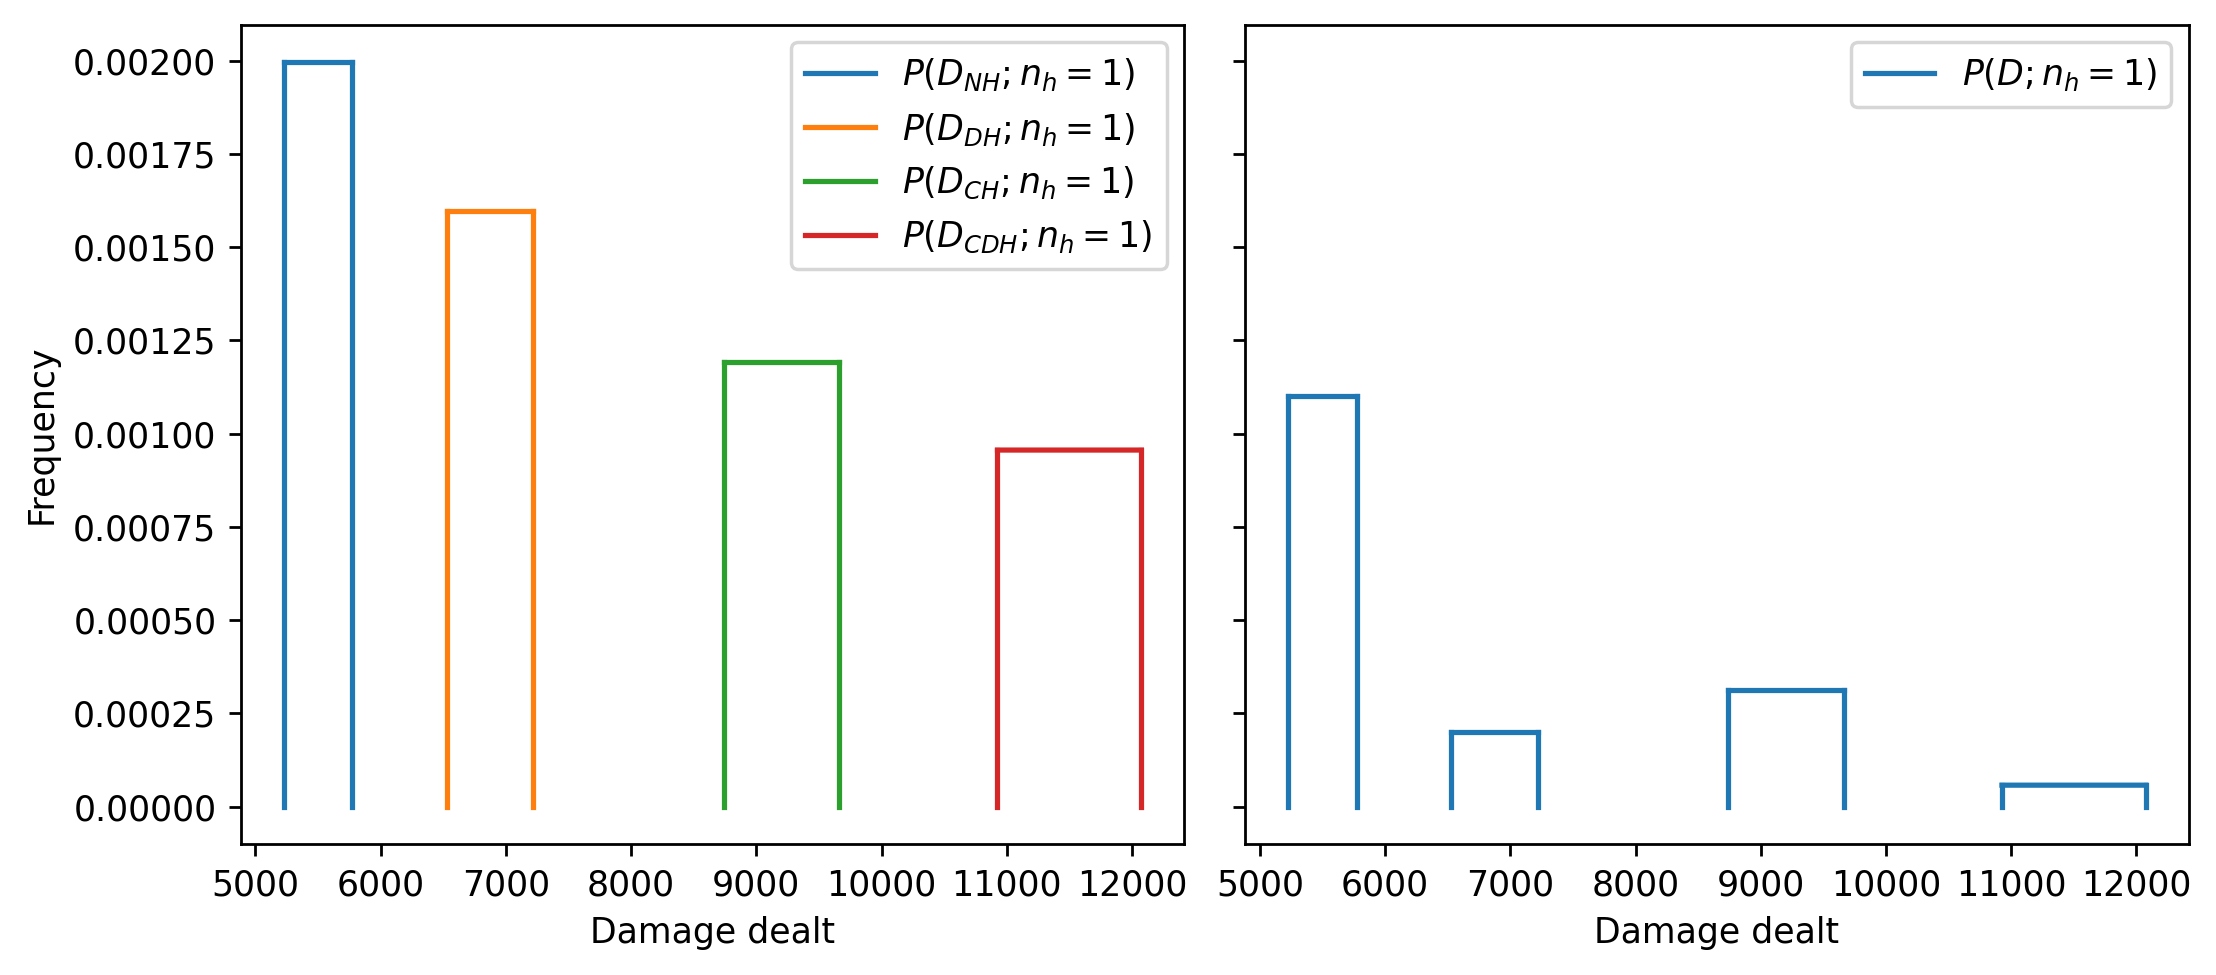
\includegraphics[width=0.95\linewidth]{img/mixture-distribution.png}
        \caption{Example of unweighted component damage distributions for a single hit (left) and the resulting mixture distribution after weighting by $p_i$ (right). The probability for each hit type is $\textbf{p} = [0.593, 0.221, 0.136, 0.050]$, $D_2 = 5,000$, and the damage modifiers are $\lambda_C = 1,621$ and $\lambda_D = 125$. A 10\% damage buff is also applied. A 10\% damage buff is also applied.}\label{fig:1-hit-mixture}
    \end{figure}

    The damage distribution for landing two hits is the sum of two 1-hit distributions, \textit{i.e.}, a sum of independent, random variables. The resulting distribution is computed by convolving two 1-hit distributions, 
    
    \begin{equation}
        P(D; n_h = 2) = P(D; n_h^\prime = 1) \ast P(D; n_h^\prime = 1)
    \end{equation}
    where $\ast$ denotes a convolution. In general, the damage distribution for landing $n_h$ hits is computed by convolving $P(D; n_h = 1)$ with itself $n_h - 1$ times, denoted in shorthand by
    
    \begin{equation}\label{eqn:damage-dist-convo}
        P(D;n_h) = P(D;n_h^\prime=1)^{\ast n_h} \stackrel{\text{def}}{=} \underbrace{P(D; n_h^\prime = 1) \ast P(D; n_h^\prime = 1) \ast\dots\ast P(D; n_h^\prime = 1)}_{n_h}
    \end{equation}
    Figure \ref{fig:convo-convergence} shows some examples of DPS distribution, $P(\dot{D}; n_h) = P(D; n_h) / t$, examples for different values of $n_{h}$.
    \begin{figure}[H]
        \centering
        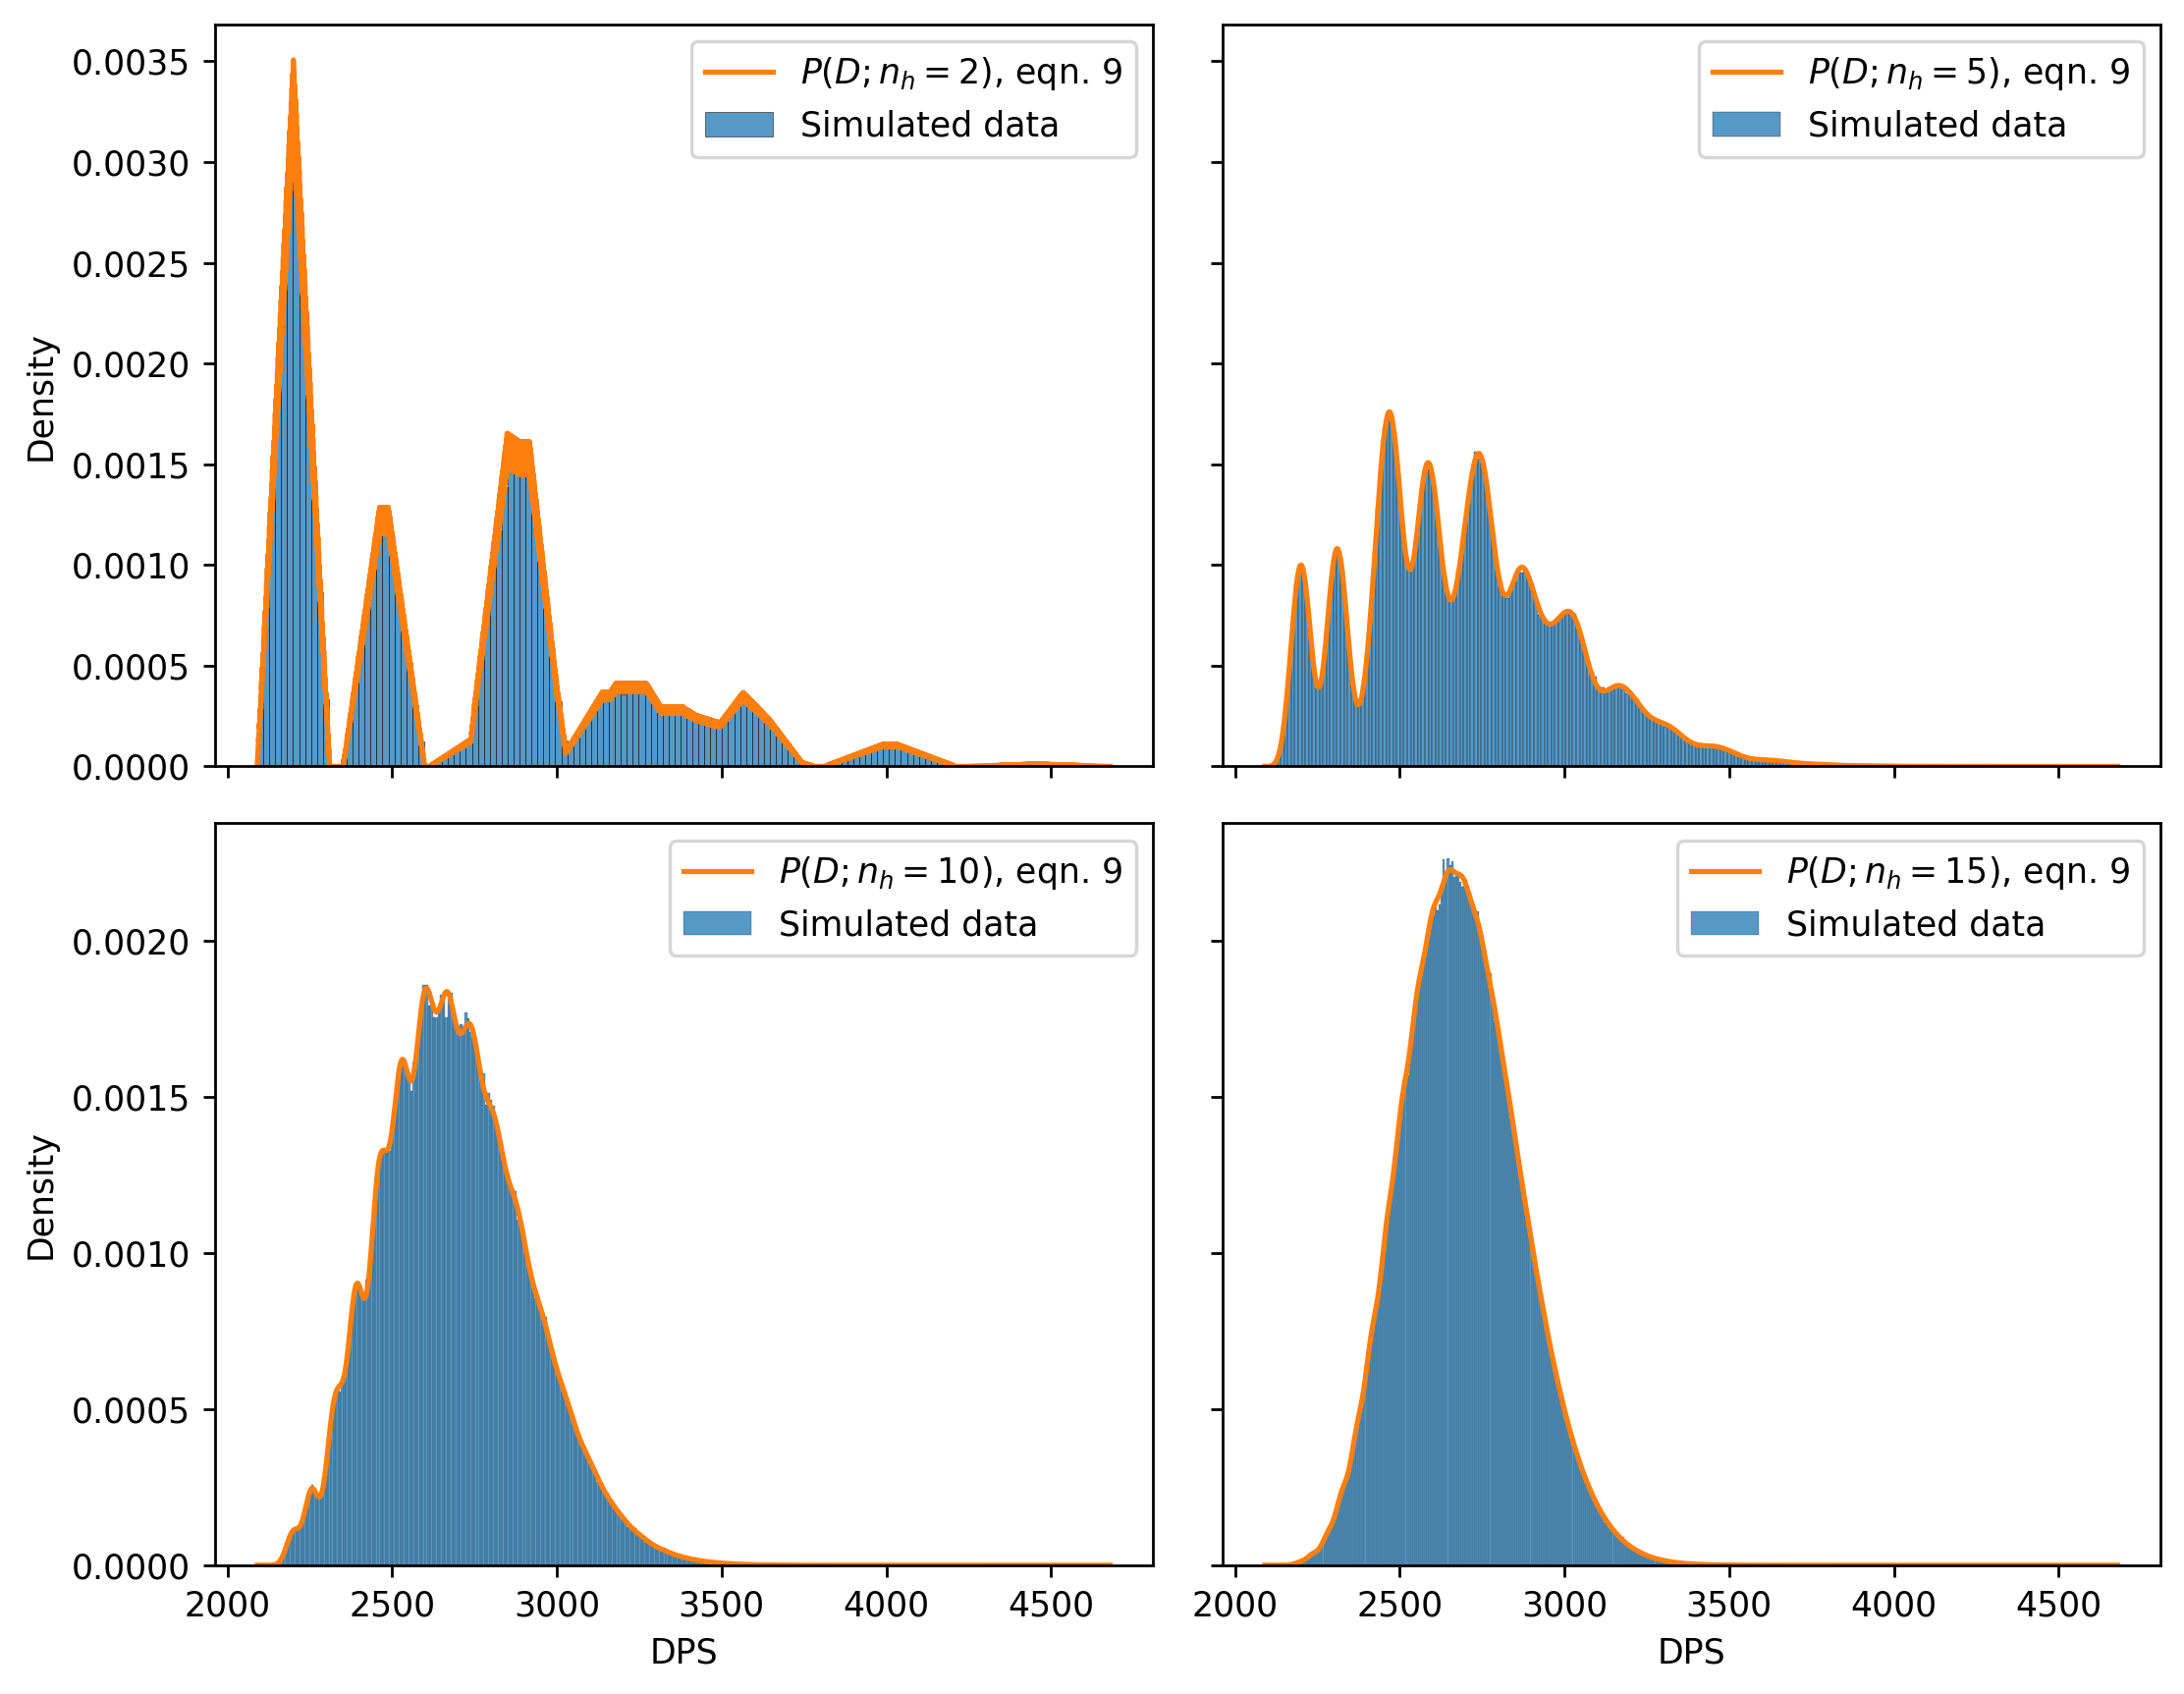
\includegraphics[width=0.95\linewidth]{img/convo-convergence.png}
        \caption{DPS distributions for a single skill with $n_{h} = 2, 5, 10,$ and $15$. The orange curves are the DPS distributions computed via eqn. \ref{eqn:damage-dist-convo} and the blue histograms are simulations with 500,000 samples each for comparison. A GCD of 2.50s is used and the total time elapsed is $t = n_h \times 2.50$s. The probability for each hit type is $\textbf{p} = [0.593, 0.221, 0.136, 0.050]$, $D_2 = 5,000$, and the damage modifiers are $\lambda_C = 1,621$ and $\lambda_D = 125$. A 10\% damage buff is also applied.}\label{fig:convo-convergence}
    \end{figure}
    An important property of $P(D; n_h)$ is that it converges to a normal distribution as $n_h \rightarrow \infty$. For the distributions in Figures \ref{fig:1-hit-mixture} and \ref{fig:convo-convergence}, $P(D, n_h)$ begins as a set of uniform distributions at $n_h = 1$. As $n_h$ grows, it transforms to a smooth, multimodal distribution, $n_h = 5$, then to a positive-skewed unimodal distribution, $n_h = 10 - 15$, and finally towards a normal distribution, $n_h > 15$. Once $n_h$ becomes large enough that it becomes unimodal, $P(D, n_h)$ can be accurately parameterized by a skew normal distribution,\footnote{See Figure \ref{fig:skew-norm-fits} in the Appendix for fit examples}
    \begin{equation}
        P_{sn}(D; \xi, \omega, \alpha) = \frac{2}{\omega \sqrt{2 \pi}} \exp\left[-\frac{(D-\xi)^{2}}{2 \omega^{2}}\right] \int_{-\infty}^{\alpha\left(\frac{D-\xi}{\omega}\right)} \frac{1}{\sqrt{2 \pi}} \exp\left[-\frac{\tau^{2}}{2}\right] d \tau
    \end{equation}
    where $\xi$ is the location, $\omega$ is the scale, and $\alpha$ is the shape. These three parameters can be expressed in terms of the first 3 moments, for which we have a means of computing exactly.\footnote{As outlined in {''Variability in damage calculations''}.} The relationship between the skew normal parameters and moments is

    \begin{equation}\label{eqn:skew-norm-params}
        \begin{split}
            \xi &= \mu - \omega \delta \sqrt{\frac{2}{\pi}} \\
            \omega &= \left(\frac{\sigma^2}{1-\frac{2\delta}{\pi}}\right)^2 \\
            \alpha &= \frac{\textrm{sgn}(\gamma)\delta}{\sqrt{1-\delta^2}} 
        \end{split}
    \end{equation}
    where
    \begin{equation}\label{eqn:delta}
        \delta = \sqrt{\frac{\pi}{2} \frac{\left|{\gamma}\right|^{\frac{2}{3}}}{\left|{\gamma}\right|^{\frac{2}{3}}+((4-\pi) / 2)^{\frac{2}{3}}}}
    \end{equation}
    and $\mu$ is the mean, $\sigma^2$ is the variance, and $\gamma$ is the skewness. This skew normal distribution accurately fits $P(D, n_h)$ for intermediate to large $n_h$ and correctly satisfies the asymptotic distribution by transforming to a normal distribution, as $\alpha \rightarrow 0$ as when $n_h \rightarrow \infty$.
    % TODO: figure out more about this relationship
    The value of $n_h$ required for a skew-normal to become a valid approximation will depend on the elements of $\textbf{p}$. If elements of $\textbf{p}$ are close to 0 or 1, $P(D; n_h)$ converges  towards a normal distribution slower than if the elements of $\textbf{p}$ are similar to each other.\footnote{This also means the multiple peaks smooths out toward a unimodal distribution more slowly.} The exact value of $n_h$ will depend on how closely the skew-normal distribution should resemble the exact damage distribution. For example, the small peaks for cases like $n_h = 10$ in Figure \ref{fig:convo-convergence} may or may not be important. In the context of FFXIV, sampling these DPS distributions requires perfectly executing the proposed rotation in an encounter. Resolving fine details in the DPS distribution will likely require thousands kills, each with a perfectly executed rotation. For practically all cases, replicating fine details will be irrelevant. 
    
    Choosing whether to compute damage distributions from convolutions or parameterizing a skew normal distribution will likely be decided by the computational cost. The convolutions can be efficiently computed via fast Fourier transforms with computational complexity $\mathcal{O}(N \log N)$, although $n_h-1$ convolutions must also be performed. Additionally, $N$ is number of integers in $\textrm{supp}[P(D;n_h)]$, which is approximately all integers from $n_h \lfloor 0.95 D_2 \rfloor$ to $n_h \lfloor 1.05 D_3 \rfloor$, where a critical-direct occurs for $D_3$. For high-potency attacks and large $n_h$, $N$ can grow quite large and convolutions become expensive. Parameterizing the skew-normal distribution requires multiplication operations on all possible hit types. The total number of ways to arrange permutations of different hit type counts that sum to $n_h$  grows combinatorically, $\binom{5n_h-1}{3}$, which scales as $\mathcal{O}(n_h^3)$. While the scaling for enumerating all hit types is worse than $\mathcal{O}(N \log N)$ for convolutions, $n_h$ is typically much smaller than $N$. The actual performance crossover will depend on scaling prefactors (which big $\mathcal{O}$ notation ignores) and the specific implementations for each method. When both methods were used to compute damage distributions with the same parameters used in Figure \ref{fig:convo-convergence} but with $n_h = 50$ and $n_h = 100$, it was found that parameterizing the skew-normal distribution was about an order of magnitude faster than the convolution method both times.\footnote{The final, 49$^\textrm{th}$, convolution for $n_h = 50$ has $N = 588,700$ where the total number of hit type permutations which sum to 50 is just $23,426 \sim n_h^3$. The difference in the number of elements is also about an order of magnitude, in agreement with the difference in computational time.}  A deeper analysis is certainly merited, but these results suggest that parameterizing a skew-normal distribution will generally be more efficient than performing $n_h-1$ convolutions when the approximation is valid.
    
   While the above examples were all for a single skill landing $n_h$ hits, damage distributions can still be computed for rotations. The rotation DPS distribution can be computed in the following steps:
    \begin{enumerate}
        \item For each skill damage distributions parameterized to a skew normal distribution, the moments for each skill distribution are computed, the skew normal parameters are computed using eqn. \ref{eqn:skew-norm-params} and eqn. \ref{eqn:delta}, and then $P_{sn}(D; \xi, \omega, \alpha)$ is computed for each skill.
        \item For damage distributions computed from convolutions, the damage distribution for each skill is separately computed. A combined convolution damage distribution is computed by convolving all skill damage distributions together.
        \item Convolve the skew normal damage distributions and combined convolution damage distribution with each other to obtain the rotation damage distribution.
    \end{enumerate}    
    To illustrate the above steps, consider a simplified White Mage rotation consisting of Glare III, Assize, Dia applications, and Dia DoT ticks. After 2 minutes and a GCD of 2.50s, the rotation is
    \begin{table}[H]
        \centering
        \begin{tabular}{@{}llll@{}}
        \toprule
        Skill              & $n_h$ & $D_2$  & Method to compute $P(D;n_h)$  \\ \midrule
        Glare III          & 44    & 9000   & Skew normal   \\
        Assize             & 3     & 9500   & Convolutions  \\
        Dia (application)  & 4     & 1500   & Convolutions  \\
        Dia (DoT tick)     & 37    & 1500   & Skew normal   \\ \bottomrule
        \end{tabular}
        \end{table}
    For all skills, the probability of each hit type is $\textbf{p} = [0.593, 0.221, 0.136, 0.050]$, the damage modifier for each hit type is $\lambda_C = 1,621$ and $\lambda_D = 125$. Figure \ref{fig:deterministic-rotation} shows the skill and rotation DPS distribution.

    \begin{figure}[H]
        \centering
        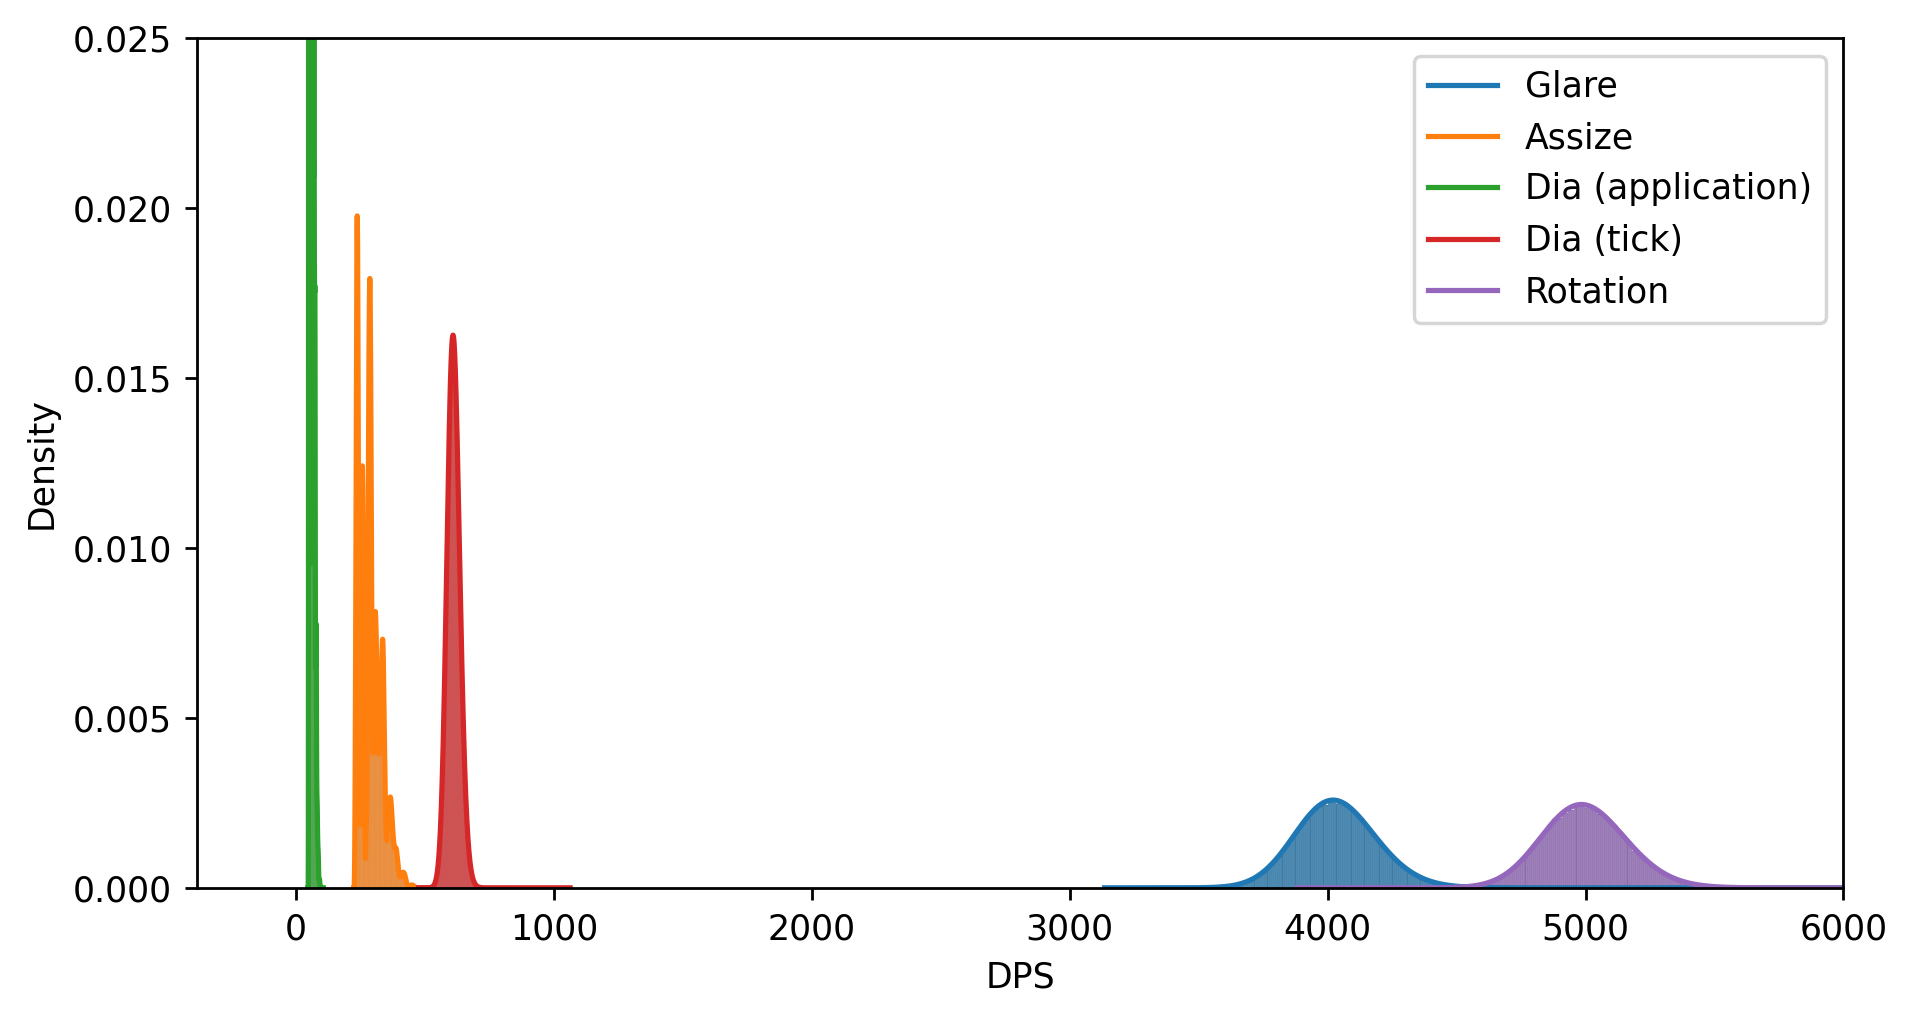
\includegraphics[width=0.95\linewidth]{img/deterministic-rotation.png}
        \caption{DPS distributions for each skill and the overall rotation. The shaded histograms are from simulations for comparison, each with 200,000 samples.}\label{fig:deterministic-rotation}
    \end{figure}
    \newpage
    \section{Stochastic rotations I: randomly distributed hit counts}
    Here, we focus on deriving damage distributions for skills and abilities whose total number of usages depend on chance. As previously mentioned, examples include Bard's Bloodletter, Pitch Perfect, and Refulgent Arrow or Astrologian's Lord of Crowns. Whether a usage of the skill/ability is granted or not often depends on a Bernoulli trial, so the total number of usages granted is also often binomially distributed. The stochastic portion of the damage distribution is a mixture distribution that averages over all possible number of usages granted,

    \begin{equation}\label{eqn:rand-skill-usage-mixture}
        P_s(D) = \sum_{k_s = k_{s,0}}^{n_s} w(k_s) P(D; n_h = k_s)  
    \end{equation}
    where $k_{s,0}$ is the minimum number usages granted (often, but not always 0), $n_s$ is the maximum number of usages granted, the weights $w(k_s)$ are the probability of $k_s$ usages being granted, and $P(D, n=k_s)$ is the resulting deterministic damage distribution when $k_s$ usages are granted. A unique feature for this class of stochastic rotations is that the stochastic and deterministic portions are neatly separable by skill/action. The deterministic portion of the damage distribution can be computed using the methods described in Section \ref{sec:deterministic} and the stochastic portion can be computed by eqn. \ref{eqn:rand-skill-usage-mixture}.
    \subsection{Example: Lord of Crowns}
    To illustrate an example of this case, consider Astrologian's Minor Arcana ability after 6 minutes has elapsed and 7 Minor Arcana cards are drawn from the divining deck.\footnote{Most other skills/actions add some additional intricacies, but still work in this framework. For example, each Refulgent Arrow proc will also reduce the total number of Burst Shot hits by 1. Furthermore, the total number of Pitch Perfect usages with 3 Repertoire stacks will often be $\lfloor k_s / 3 \rfloor$ plus an additional Pitch Perfect where the number of Repertoire stacks is the modulus.} Each Minor Arcana draw has a $50\%$ chance of drawing a Lord of Crowns (250 potency of damage dealt) or Lady of Crowns (0 potency of damage dealt), so the number of Lord of Crowns drawn will be binomially distributed,
    
    \begin{equation}\label{eqn:lord-of-crowns-weights}
        w(k_s) = P_B(k_s; p_{s}, n_s) = \binom{n_s}{k_s} p_s^{k} (1-p_s)^{n_s-k_s}
    \end{equation}
    where $p_s$ is the success rate of drawing a card and $n_s$ is the maximum number of successes. Eqn. \ref{eqn:lord-of-crowns-weights} yields the weights for eqn. \ref{eqn:rand-skill-usage-mixture}, but the damage distributions for landing $k_s$ hits is also required. Since $n_s$ is small, the damage distribution will still be multi-modal and is exactly computed by convolutions, \ref{eqn:damage-dist-convo}. Finally, the base damage for Lord of Crowns is assumed to be $D_2 = 6,000$, the probabilities for different hit types is $\textbf{p} = [0.78, 0.21, 0.01, 1.9 \times 10^{-3}]$ and the damage modifiers for each hit type is $\lambda_C = 1,567$ and $\lambda_D = 125$. Figure \ref{fig:hit-enumeration} shows the component damage distribution for landing $0 - 7$ hits, computed via convolutions, and the respective probability of landing that number of hits.

    \begin{figure}[H]
        \centering
        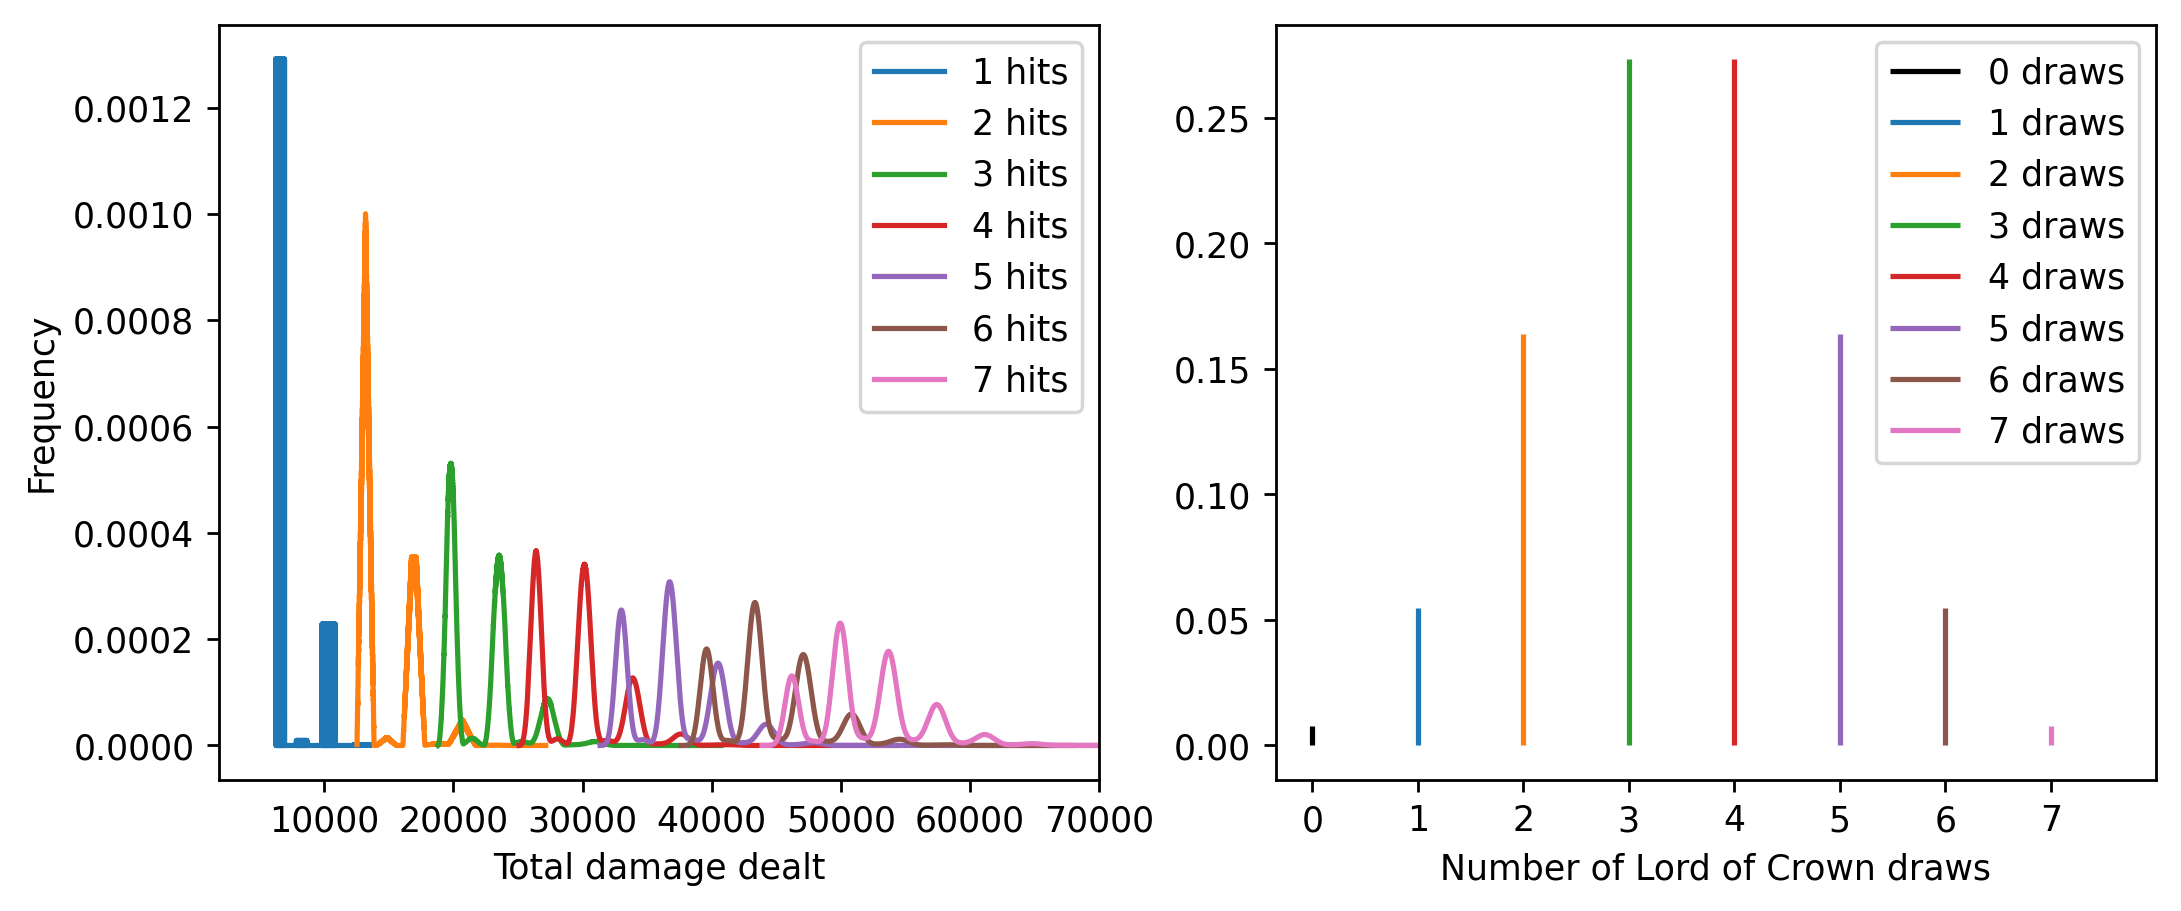
\includegraphics[width=0.99\linewidth]{img/hit-enumeration.PNG}
        \caption{Damage distribution when Lord of Crowns lands $1 - 7$ hits (left) and the probability of drawing $0-7$ Lord of Crowns (right). The damage distribution for $k_s = 0$ is omitted for clarity.}\label{fig:hit-enumeration}
    \end{figure}

    Eqn. \ref{eqn:rand-skill-usage-mixture} can now be used to compute the stochastic damage distribution, which accounts for variability from hit types, damage rolls, and the total number of hits. The stochastic damage distribution can also be compared against a similar deterministic damage distribution. The average number of Lord of Crowns draws is $n_s \times p_s = 7 \times 0.5 = 3.5$ and the two closest integer number of Lord of Crown draws are 3 and 4. Figure \ref{fig:avg-rotation} shows the DPS distributions for all cases.

    \begin{figure}[H]
        \centering
        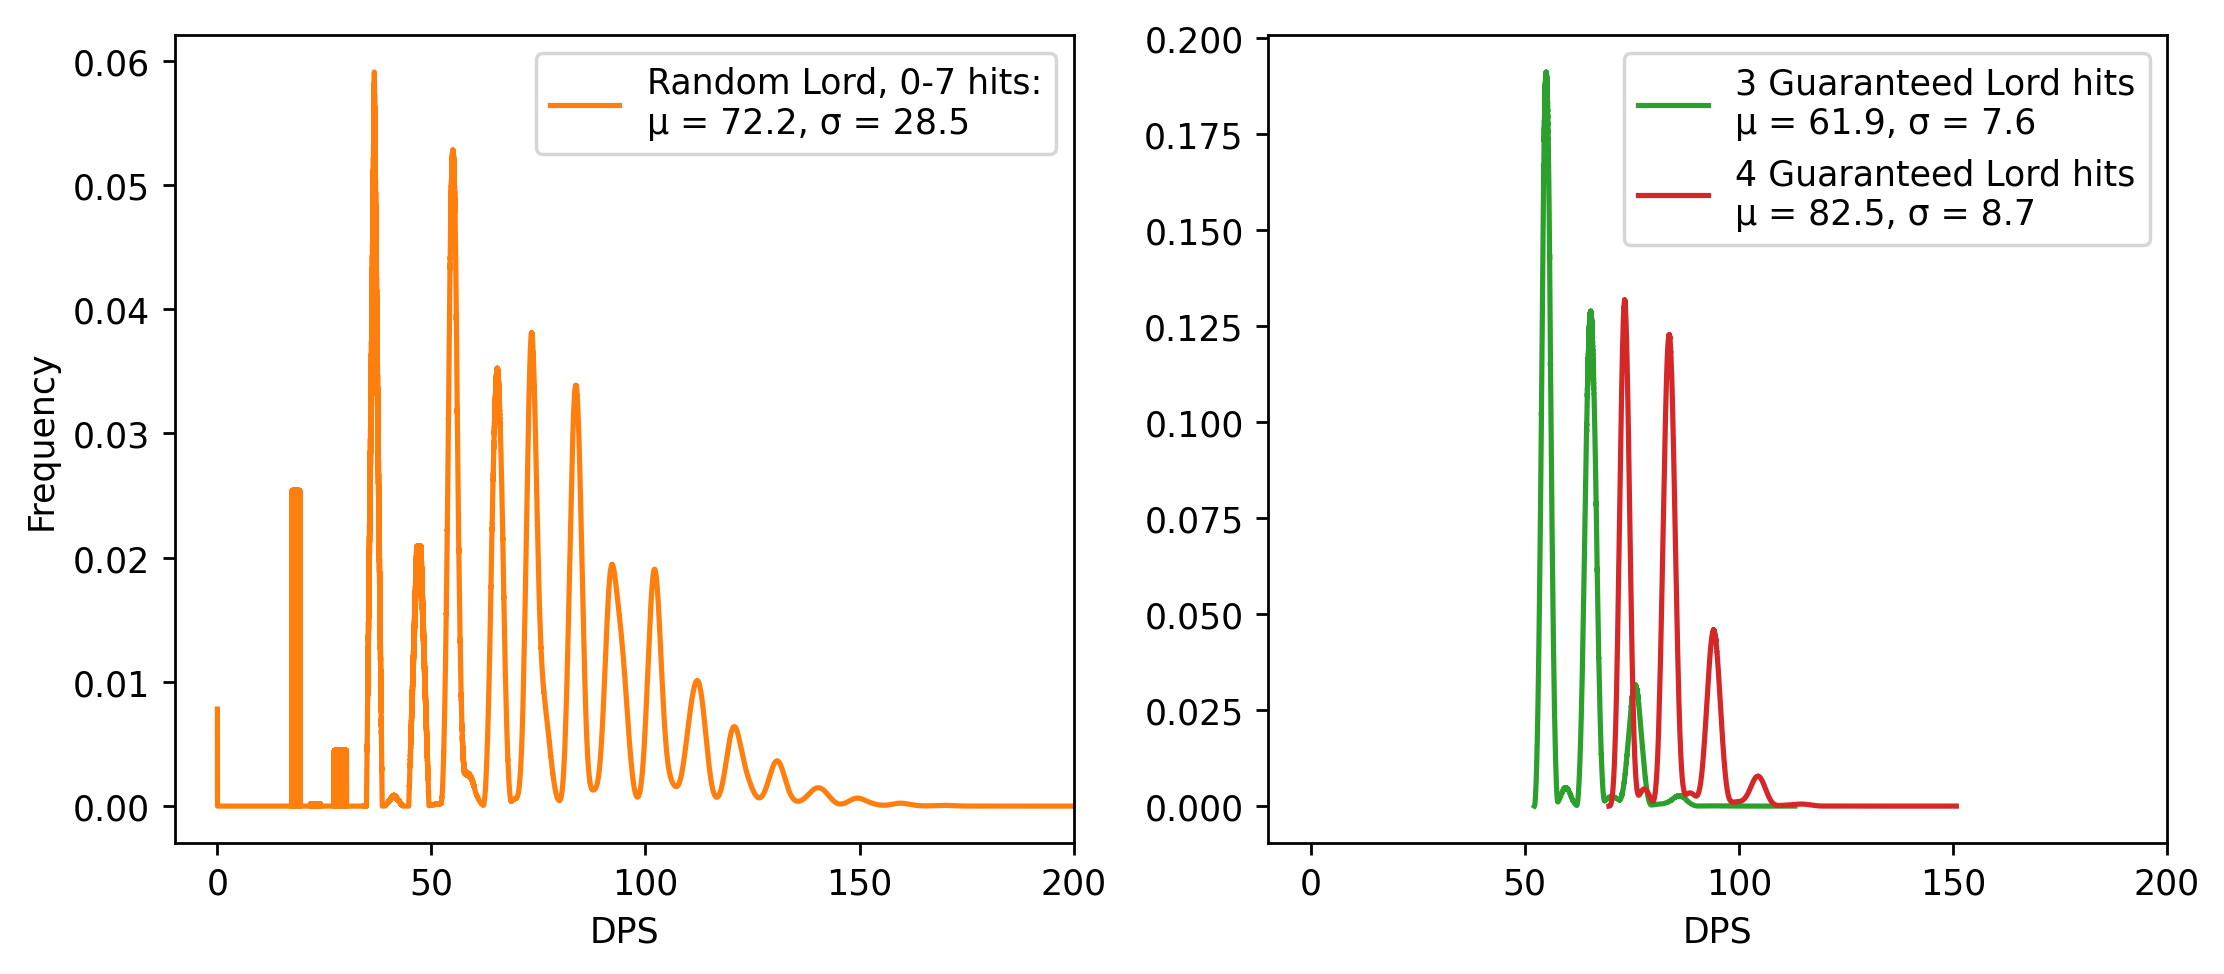
\includegraphics[width=0.99\linewidth]{img/averaged-rotation.png}
        \caption{The DPS distribution when Lord of Crowns has a 50\% chance of being drawn and landing $0 - 7$ hits (left) and the DPS distributions when Lord of Crowns is guaranteed, but lands either 3 or 4 hits (right).}\label{fig:avg-rotation}
    \end{figure}
    Unsurprisingly, the average DPS when Lord of Crowns draws are random is somewhere between the average DPS for 3 and 4 guaranteed hits, but the standard deviation is about 3 times larger. This is expected since there can be 0, 1, 2, 5, 6 or 7 lord draws, which will deal significantly different amounts of damage compared to the average number of draws. While the random nature of drawing Lord of Crowns introduces additional variability into the DPS distribution, the absolute amount of variability is fairly small compared to DPS variance from combust ticks and malefic casts.
    
    The rotation damage distribution can be computed by following the same steps used to compute the rotation damage distribution for deterministic rotations -- the convolutions are agnostic to the particular form of the damage distribution for each skill. For a 2.50s GCD and using the same stats for the Lord of Crown calculation, the rotation and method for computing each skill damage distribution is
    \begin{table}[H]
        \centering
        \begin{tabular}{@{}llll@{}}
        \toprule
        Action         & $n_h$                        & $D_2$   & Method to compute $P(D;n_h)$ \\ \midrule
        Fall Malefic   & 133                          & 6,000    & Skew normal                  \\
        Combust (tick) & 120                          & 1,375    & Skew normal                  \\
        Lord of Crowns & $P_B(k_s; p_{s}=0.5, n_s=7)$ & 6,000    & Convolutions                 \\ \bottomrule
        \end{tabular}
    \end{table}
    The skill and rotation DPS distributions are shown in Figure \ref{fig:loc-full-rotation}.
    \begin{figure}[H]
        \centering
        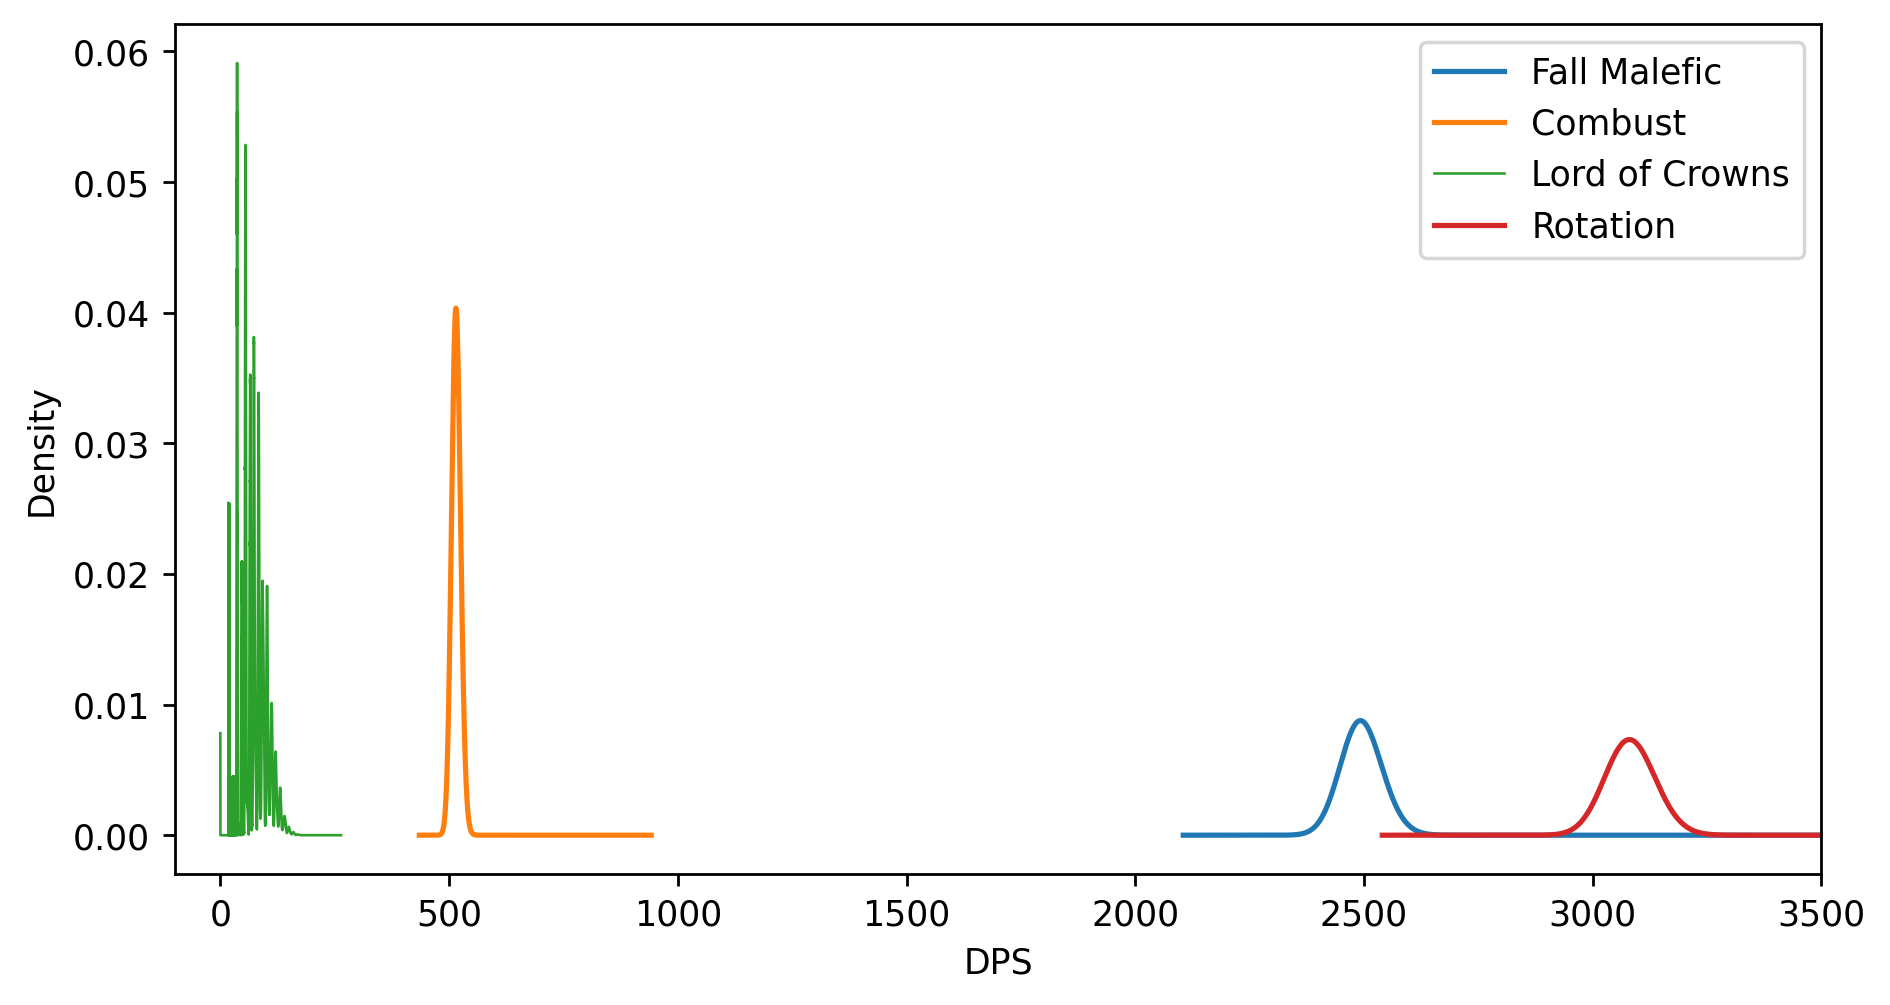
\includegraphics[width=0.95\linewidth]{img/lord-of-crowns-rotation.png}
        \caption{Skill and rotation DPS distributions for an Astrologian landing a randomly distributed number of Lord of Crown hits.}\label{fig:loc-full-rotation}
    \end{figure}
    \newpage
    \section{Stochastic rotations II: randomly distributed buff effects}
    Randomly distributed buffs are a more pervasive scenario because they affect every skill and action performed under their duration. Some examples include Astrologian's Astrodyne and the recipient of an Astrologian's Card. The damage dealt and potentially the skills performed for a rotation will randomly depend on the sequence of buffs received. As a motivating example, Astrologian's Astrodyne ability has three potential outcomes depending on the number of unique seals: no effect to damage (1 unique seal), a haste buff (2 unique seals) and a damage and haste buff (3 unique seals). For a given total number of usages, all possible buff sequences can be described with a weighted and directed tree, $T$. 
    
    The tree begins with a single node with edges directed towards three nodes, which corresponds to the three outcomes of attaining 1, 2, or 3 unique seals. Each of the three nodes has three edges directed to three additional outcome nodes. The total number of levels $T$ has is equal to the number of times the buff is executed. An example for the two usages of Astrodyne is shown in Figure \ref{fig:rotation-tree}.

    \begin{figure}[H]
        \centering
        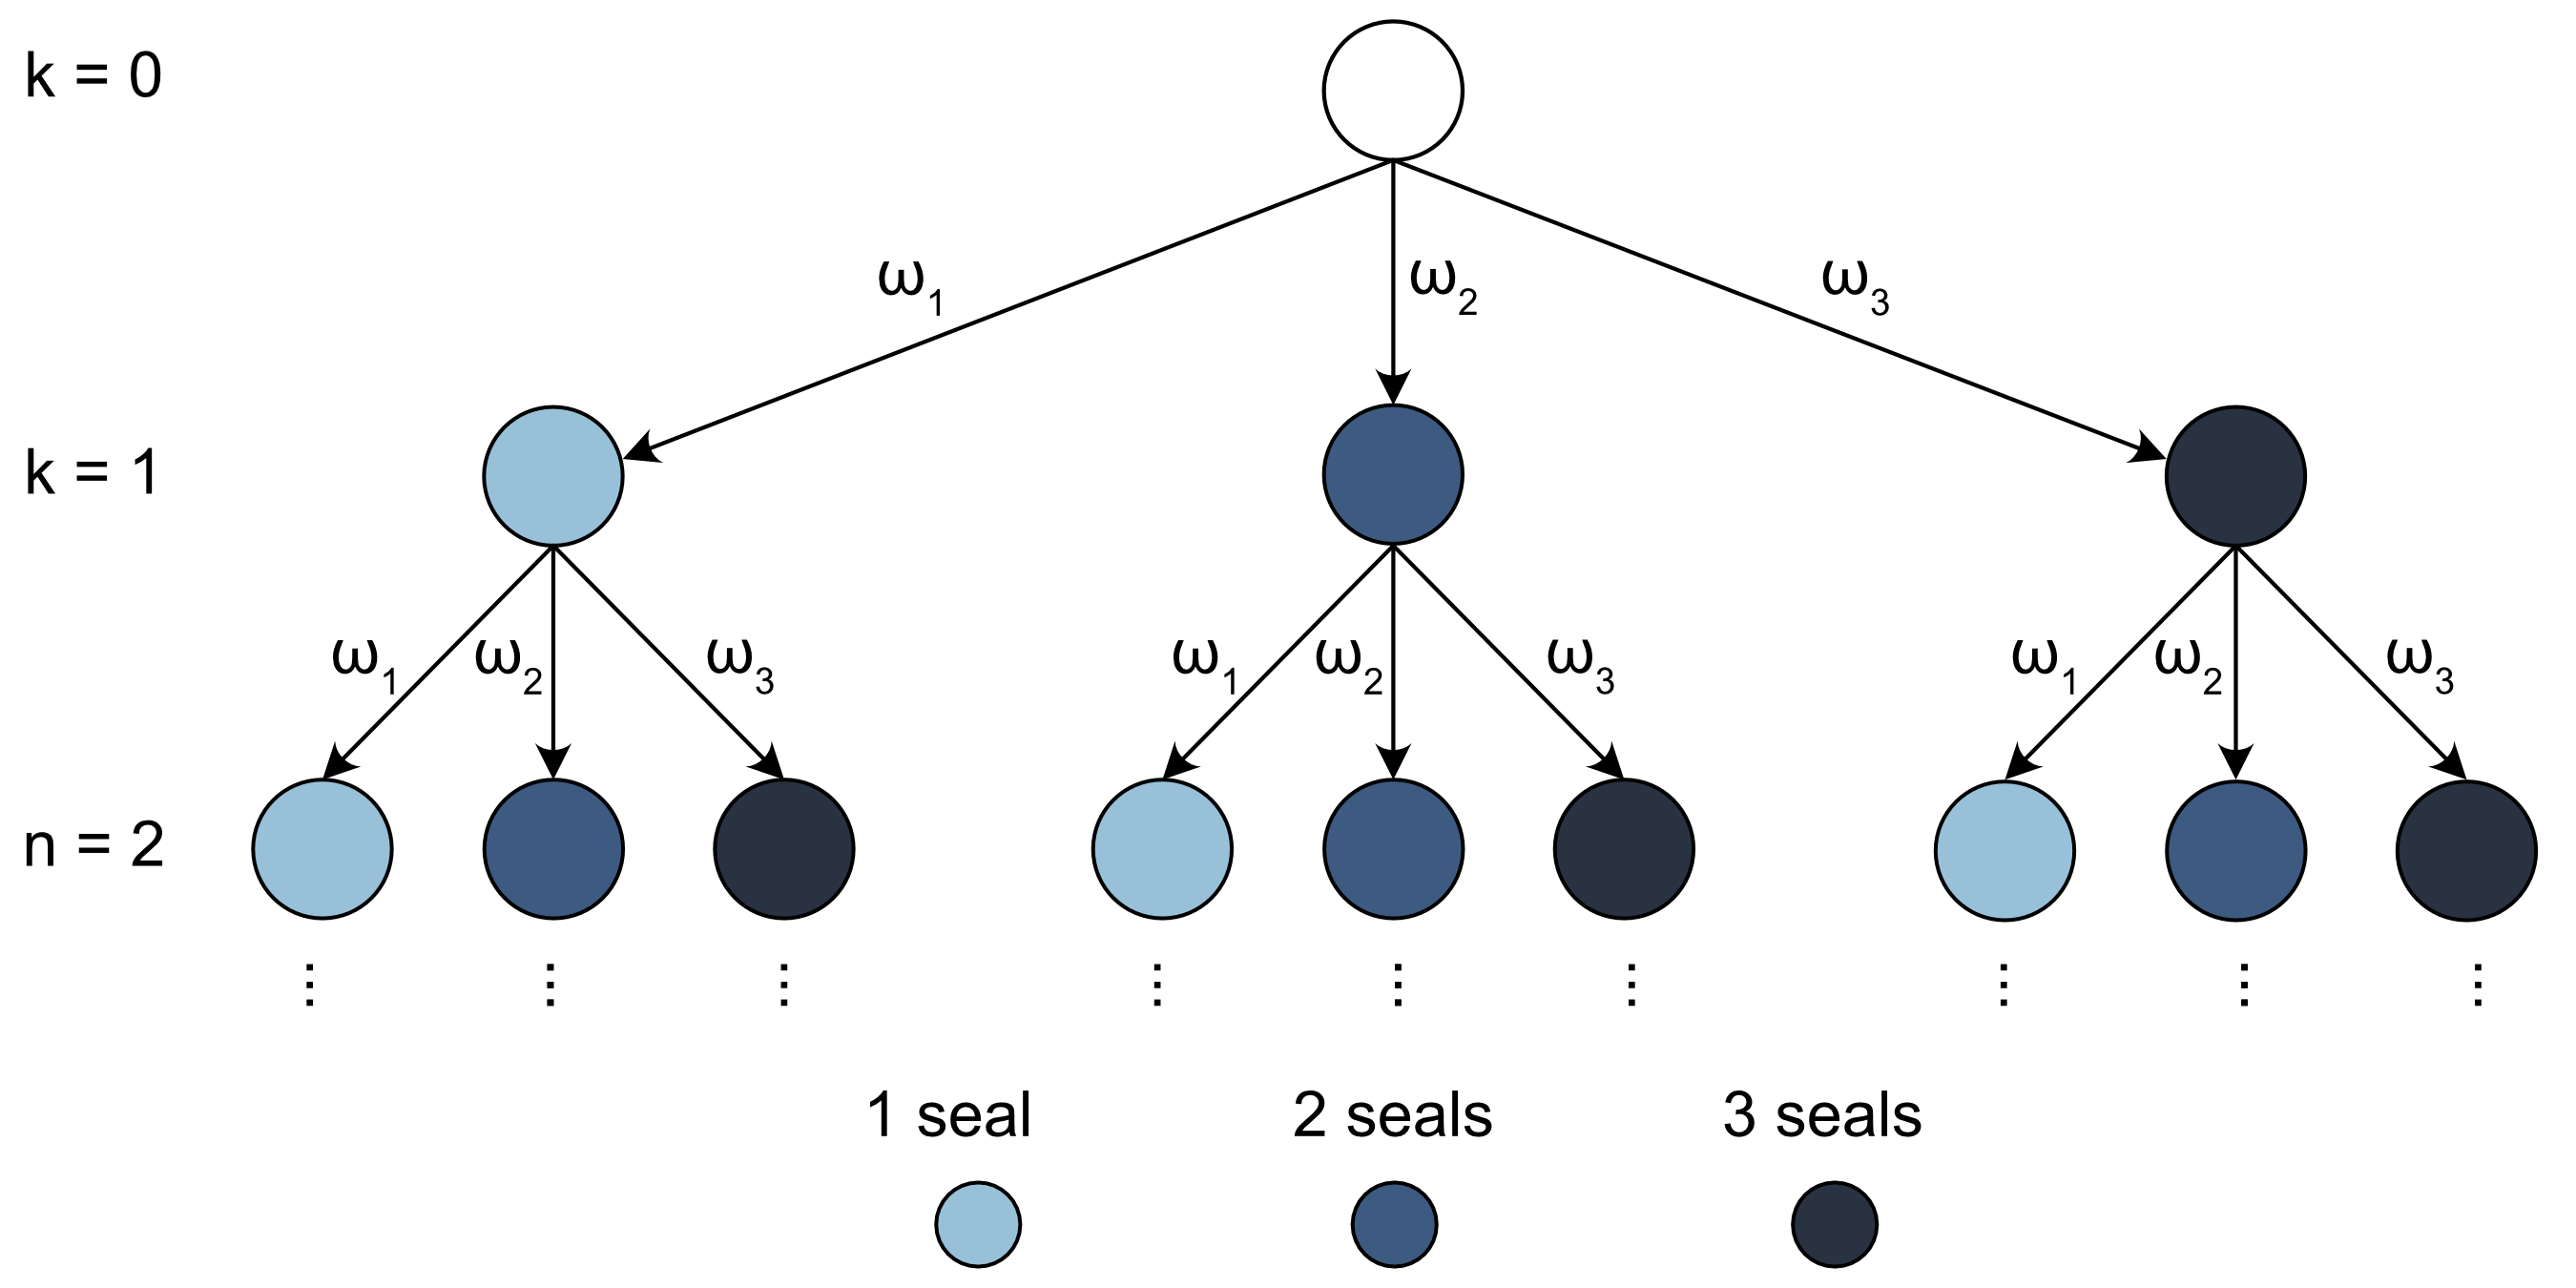
\includegraphics[width=0.9\linewidth]{img/rotation-tree.png}
        \caption{Tree graph illustrating all possible outcomes for attaining $1 - 3$ unique seals when Astrodyne is used twice.}\label{fig:rotation-tree}
    \end{figure}

    The weights $\omega_i$ are the probability of attaining $i$ unique seals. The particular values of $\omega_i$ will depend on the drawing strategy and potentially the party composition. Any particular sequence of $i$-seal Astrodynes can described by simple path $S$, which traverses from the top of the tree ($k=0$) to the bottom ($k=2$). The probability of sampling a path is given by the product of all the weights along the path,

    \begin{equation}\label{eqn:edge-prob}
        w_S = \prod_{i \in E(S)} \omega_i
    \end{equation}
    where $E(S)$ are the edges in path $S$ and $\omega_i$ is the corresponding edge weight. The overall DPS distribution can be computed by averaging over all possible simple paths, $\{S\}$,

    \begin{equation}\label{eqn:buff-weighted-P}
        P_s(D; \{S\}) = \sum_{I \in \{S\}} w_I P_I(D)
    \end{equation}
    where $P_I(D)$ is the resulting damage distribution from path $I$ and $w_I$ is defined by eqn. \ref{eqn:edge-prob}.

    \subsection{Example: simplified Astrodyne}
    
    
    To illustrate eqn. \ref{eqn:buff-weighted-P}, we once again consider an Astrologian after 6:30 minutes of a fight have elapsed. Assuming they used their Astrodyne ability every 90 seconds, there will be 5 Astrodyne usages. For the sake of demonstration, the haste buff from Astrodyne will also last 20 seconds and provide a 20\% haste buff. For 2.50s GCD, the haste buff yields two additional spell cast. This change is made only for ease of illustration the method and counting the number of additional casts granted. While this particular example will not generate damage distributions representative of the true buff effects, the strategy for averaging over all possible Astrodyne sequences.

    The rotation will solely consist of Fall Malefic casts, with $D_2 = 5,000$. The probabilities for different hit types is $\textbf{p} = [0.78, 0.21, 0.01, 1.9 \times 10^{-3}]$ and the damage modifiers for each hit type is $\lambda_C = 1,567$ and $\lambda_D = 125$. The base rotation with no Astrodyne usages will have 156 Fall Malefic casts. Each 2-seal and 3-seal Astrodyne will provide 2 additional Fall Malefic casts and each 3-seal Astrodyne will increase the damage dealt of 10 Fall Malefic hits by 5\%. Finally, the probabilities for attaining $i$ seals are
    \begin{table}[H]
        \centering
        \begin{tabular}{@{}ll@{}}
        \toprule
        Number of unique seals & probability \\ \midrule
        1                      & 0.005       \\
        2                      & 0.435       \\
        3                      & 0.560       \\ \bottomrule
        \end{tabular}
    \end{table}
    which are the probabilities when Redraw is used if the initial draw did not increase the number of unique seals. Table \ref{t:astrodyne-seq} shows the total number of hits for some examples of different Astrodyne sequences and the number of hits.
    \begin{table}[H]
        \caption{Examples of different Astrodyne sequences and their rotation}\label{t:astrodyne-seq}
        \centering
        \begin{tabular}{@{}llll@{}}
        \toprule
                    & 1, 1, 1, 1, 1 & 3, 2, 3, 1, 2 & 1, 2, 3, 2, 1 \\ \midrule
        Fall Malefic           & 156           & 144           & 152           \\
        Fall Malefic, 5\% buff & 0             & 20            & 10            \\ \midrule
        Total                  & 156           & 164           & 162           \\ \bottomrule        
        \end{tabular}
    \end{table}

    The damage distribution computed by parameterizing a skew normal distribution when $n_h > 20$ for a skill and is computed by convolutions otherwise.\footnote{Note that Fall Malefic and Fall Malefic with a 5\% damage buff are counted separately because their 1-hit damage distributions are different.} For 3 Astrodyne outcomes and 5 hits, there are 243 unique Astrodyne sequences. Figure \ref{fig:random-buff-all-avg} shows the overall damage distribution, computed by eqn. \ref{eqn:buff-weighted-P}, and all 243 component distributions.\footnote{It should be stressed that the DPS distributions for each Astrodyne sequence have significantly different means because 2 additional Fall Malefic casts are granted each time a haste buff is attained. While this certainly illustrates the importance of not dropping Malefic casts, the realistic haste effect from Astrodyne will yield damage distributions with more similar means.}
    \begin{figure}[H]
        \centering
        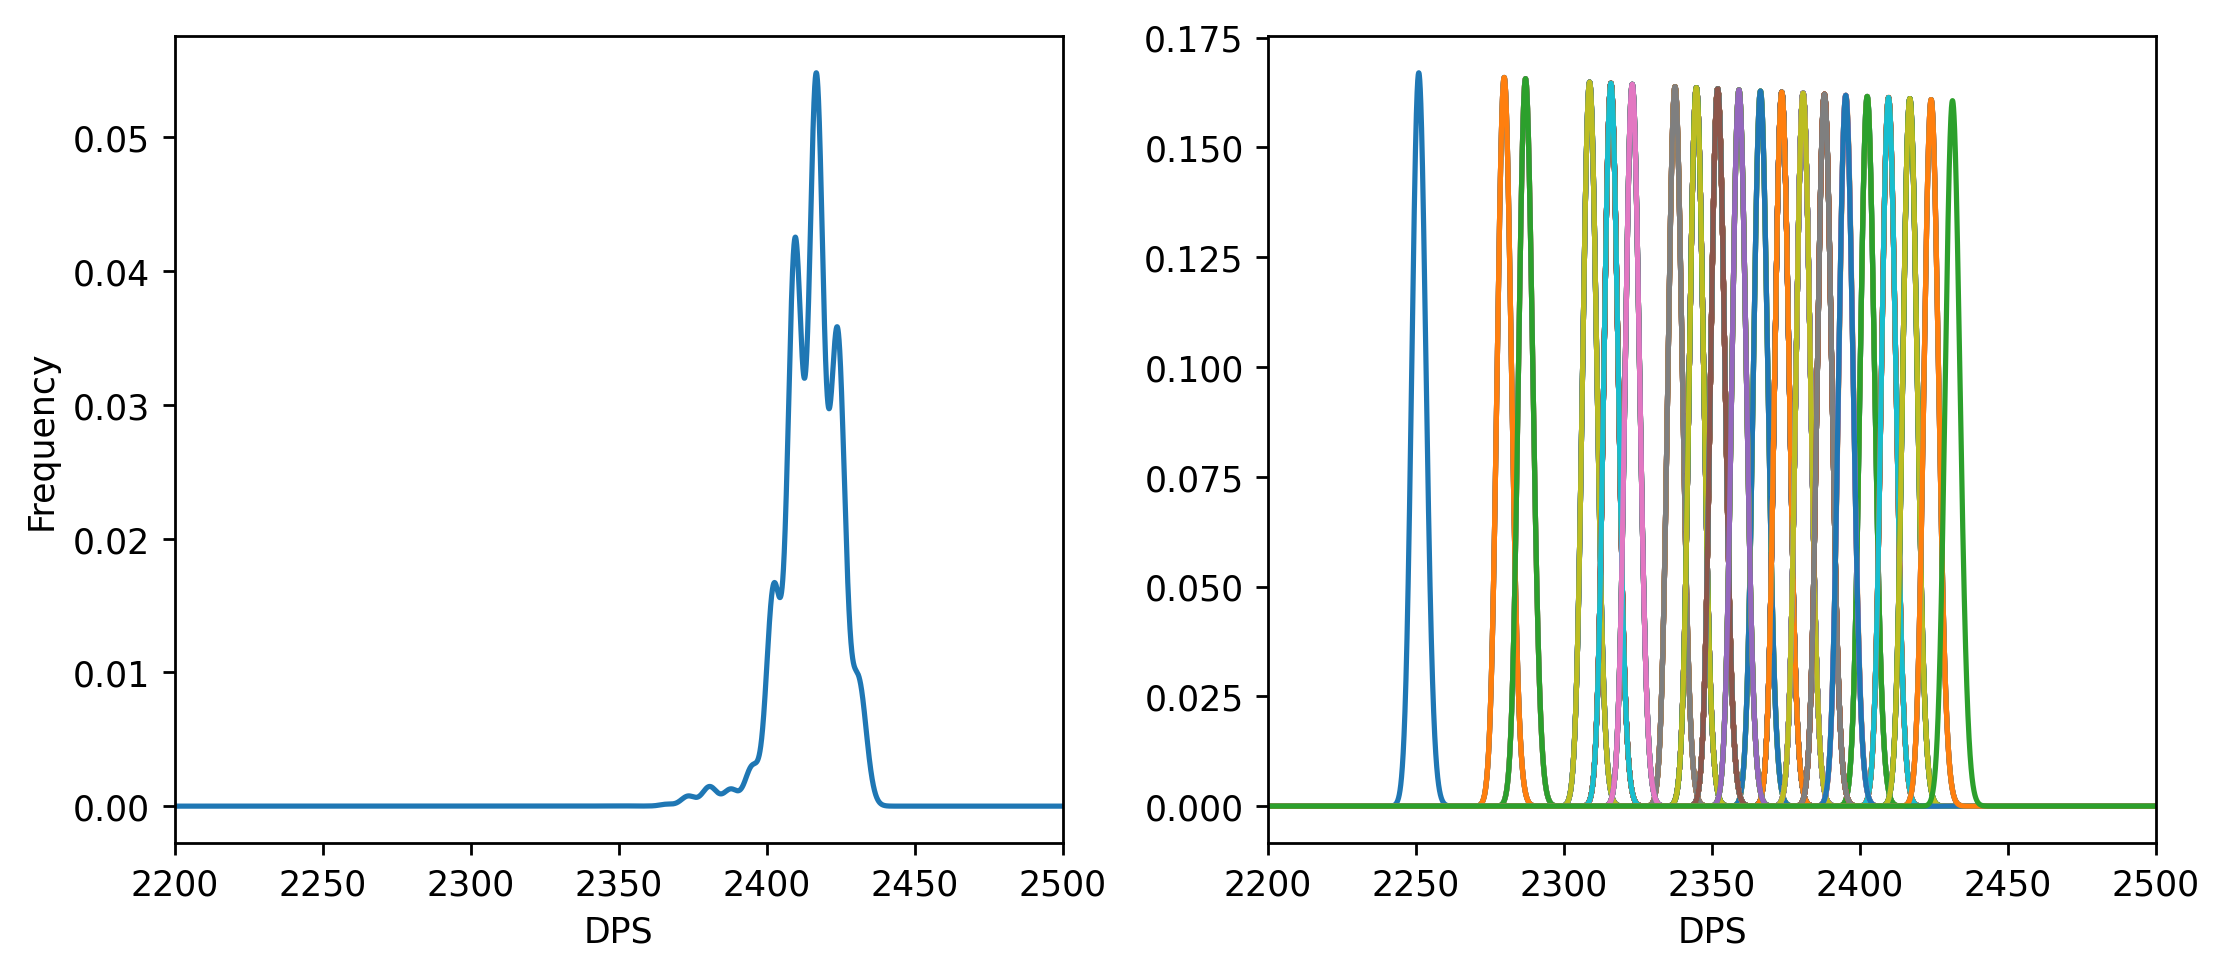
\includegraphics[width=0.95\linewidth]{img/astrodyne-all-paths.PNG}
        \caption{Overall DPS after 6:30 elapsed and 5 Astrodyne usages (left) where the component damage distributions are from all possible seal sequences (right).}\label{fig:random-buff-all-avg}
    \end{figure}


    One potential issue is that averaging the damage distribution over $\{S\}$ has become a much more computationally expensive endeavor than simply calculating a single damage distribution. When a buff has $a$ outcomes and $n$ usages, there will be $a^n$ simple paths to compute damage distributions for. The exponential growth of paths quickly leads to a computationally intractable problem. For example, a card recipient can either receive a card or not ($a=2$) every 30 seconds. Lengthy fights like ultimates can last for over 16:00, resulting in over $n = 30$ Draw usages. This leads to ca. $10^9$ unique paths, each of which requires computing a damage distribution.     
    
    However, Figure \ref{fig:random-buff-all-avg} suggests that enumerating every unique path and computing the associated damage distribution might not be required. It can be seen that the damage distributions collapse down to a handful of cases whose count is much smaller than the total number of unique Astrodyne sequences. For this pathologically simple example, the total number of 1-, 2-, and 3-seal Astrodynes used after 5 minutes is what determines the damage distribution, not their particular sequence. For example, the rotation (and damage distribution) from an Astrodyne sequence with 1, 2, 2, 3, and 3 unique seals is indistinguishable from a rotation from an Astrodyne sequence with 3, 2, 1, 2, and 3 unique seals. 
    % Permutation: sequence matters
    % Combination: sequence doesn't matter
    For 3 outcomes and 5 usages, there are 21 unique seal count \textit{combinations}, about an order of magnitude fewer than the number of sequence path \textit{permutations}. Eqn. \ref{eqn:buff-weighted-P} can be rewritten in terms of the number of unique combinations,
    \begin{equation}
        P_s(D; \{\hat{s}\}) = \sum_{i \in \{\hat{s}\}} n_i w_i P_i(D)
    \end{equation}
    where $\{\hat{s}\}$ is the set of all unique seal count combinations, $n_i$ is the number of different sequence path permutations with the same seal count combination, and $w_i$ is the probability of attaining the seal count combination $i$. The number of combinations for each unique seal count permutation still needs to be known to properly weight the mixture distribution, but enumerating all seal sequence permutations is substantially cheaper than computing every damage distribution. Figure \ref{fig:random-buff-unique} shows the same overall damage distribution, but computed using only 21 component damage distributions.\footnote{The entire damage distribution is computed for each Astrodyne sequence. In principle, it is possible to separate the stochastic and deterministic portions of the rotation damage distribution to prevent recomputing the deterministic portion damage distribution portion for each component distribution. While this is simple for this example where the haste buff nets 2 additional Fall Malefic casts, a realistic rotation damage distribution with a full party is unlikely to neatly partition into stochastic and deterministic portions that are the same across all component distributions. This strategy will likely be possible for Card recipients, as the buff only affects damage dealt.}
    \begin{figure}[H]
        \centering
        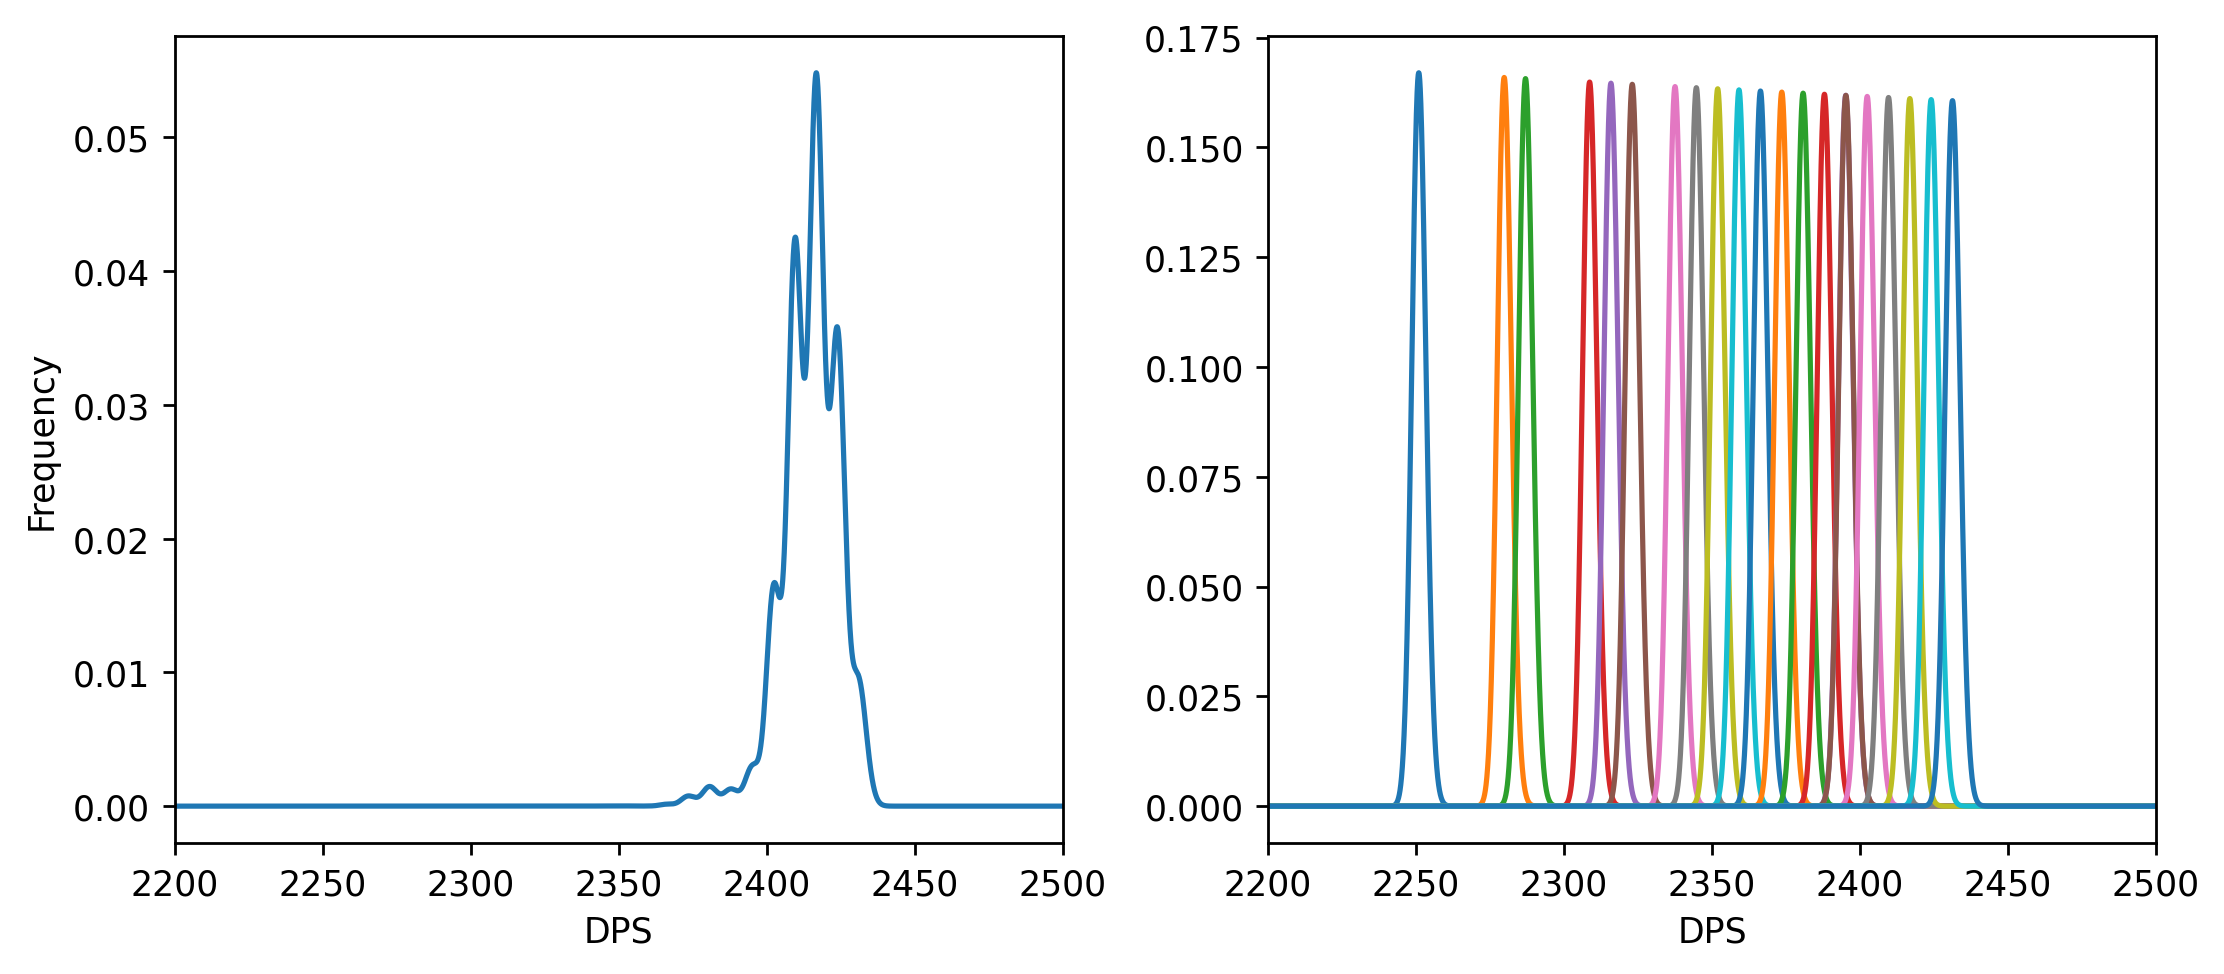
\includegraphics[width=0.95\linewidth]{img/astrodyne-unique.PNG}
        \caption{Overall DPS after 6:30 elapsed and 5 Astrodyne usages (left) where the component damage distributions are from all \textit{unique} seal count combinations (right).}\label{fig:random-buff-unique}
    \end{figure}
    Another way to further reduce the number of damage distribution computations is to ignore component distributions with exceedingly small weights. There are about 9 component distributions with means between 2250 - 2350 DPS, but their contribution is invisible in the final mixture. Indeed, the sum of weights for the first 9 component distributions is only $2 \times 10^{-4}$ (the sum of all weights is 1). A systematic method to cull unimportant components is to sort the weights from smallest to largest and only include the subset largest weights which sums to some threshold, \textit{e.g.}, 0.99. Operationally, this omits seal count combinations which are exceedingly unlikely.
    % The number of unique component damage distributions for Astrodyne will depend on the number of usages and the ability. 
    
    For realistic rotations that also includes raid buffs from a full party, the damage distributions from different Astrodyne sequences that have the same total number of $i$-seal Astrodyne usages will likely be be approximately similar, but not exactly the same. Action drift from differing GCDs and constraints imposed by encounter design can lead to small differences in damage dealt between burst phases. However, most job rotations repeat after 1 minute or 2 minutes and focus on aligning raid buffs for maximum effect, so these differences will likely remain small. The validity of this approximation is certainly an area for future exploration.
    
    Finally, the other example of a buff with randomly distributed effects is for Card recipients. Every time a card is played, a recipient can either receive a card or not receive a card. The number of unique component damage distributions will also depend on the set of eligible card recipients and their priority, the redraw strategy, and when the card is played. Card recipients will typically cards in 30 second intervals and most jobs' rotations loop after 1 minute or 2 minutes. Depending on the job, there will likely be around 4 unique component damage distributions, occurring in 30 second intervals (0:30, 1:00, 1:30, or 2:00).

    \newpage
    \section*{Appendix}
    \begin{figure}[H]
        \centering
        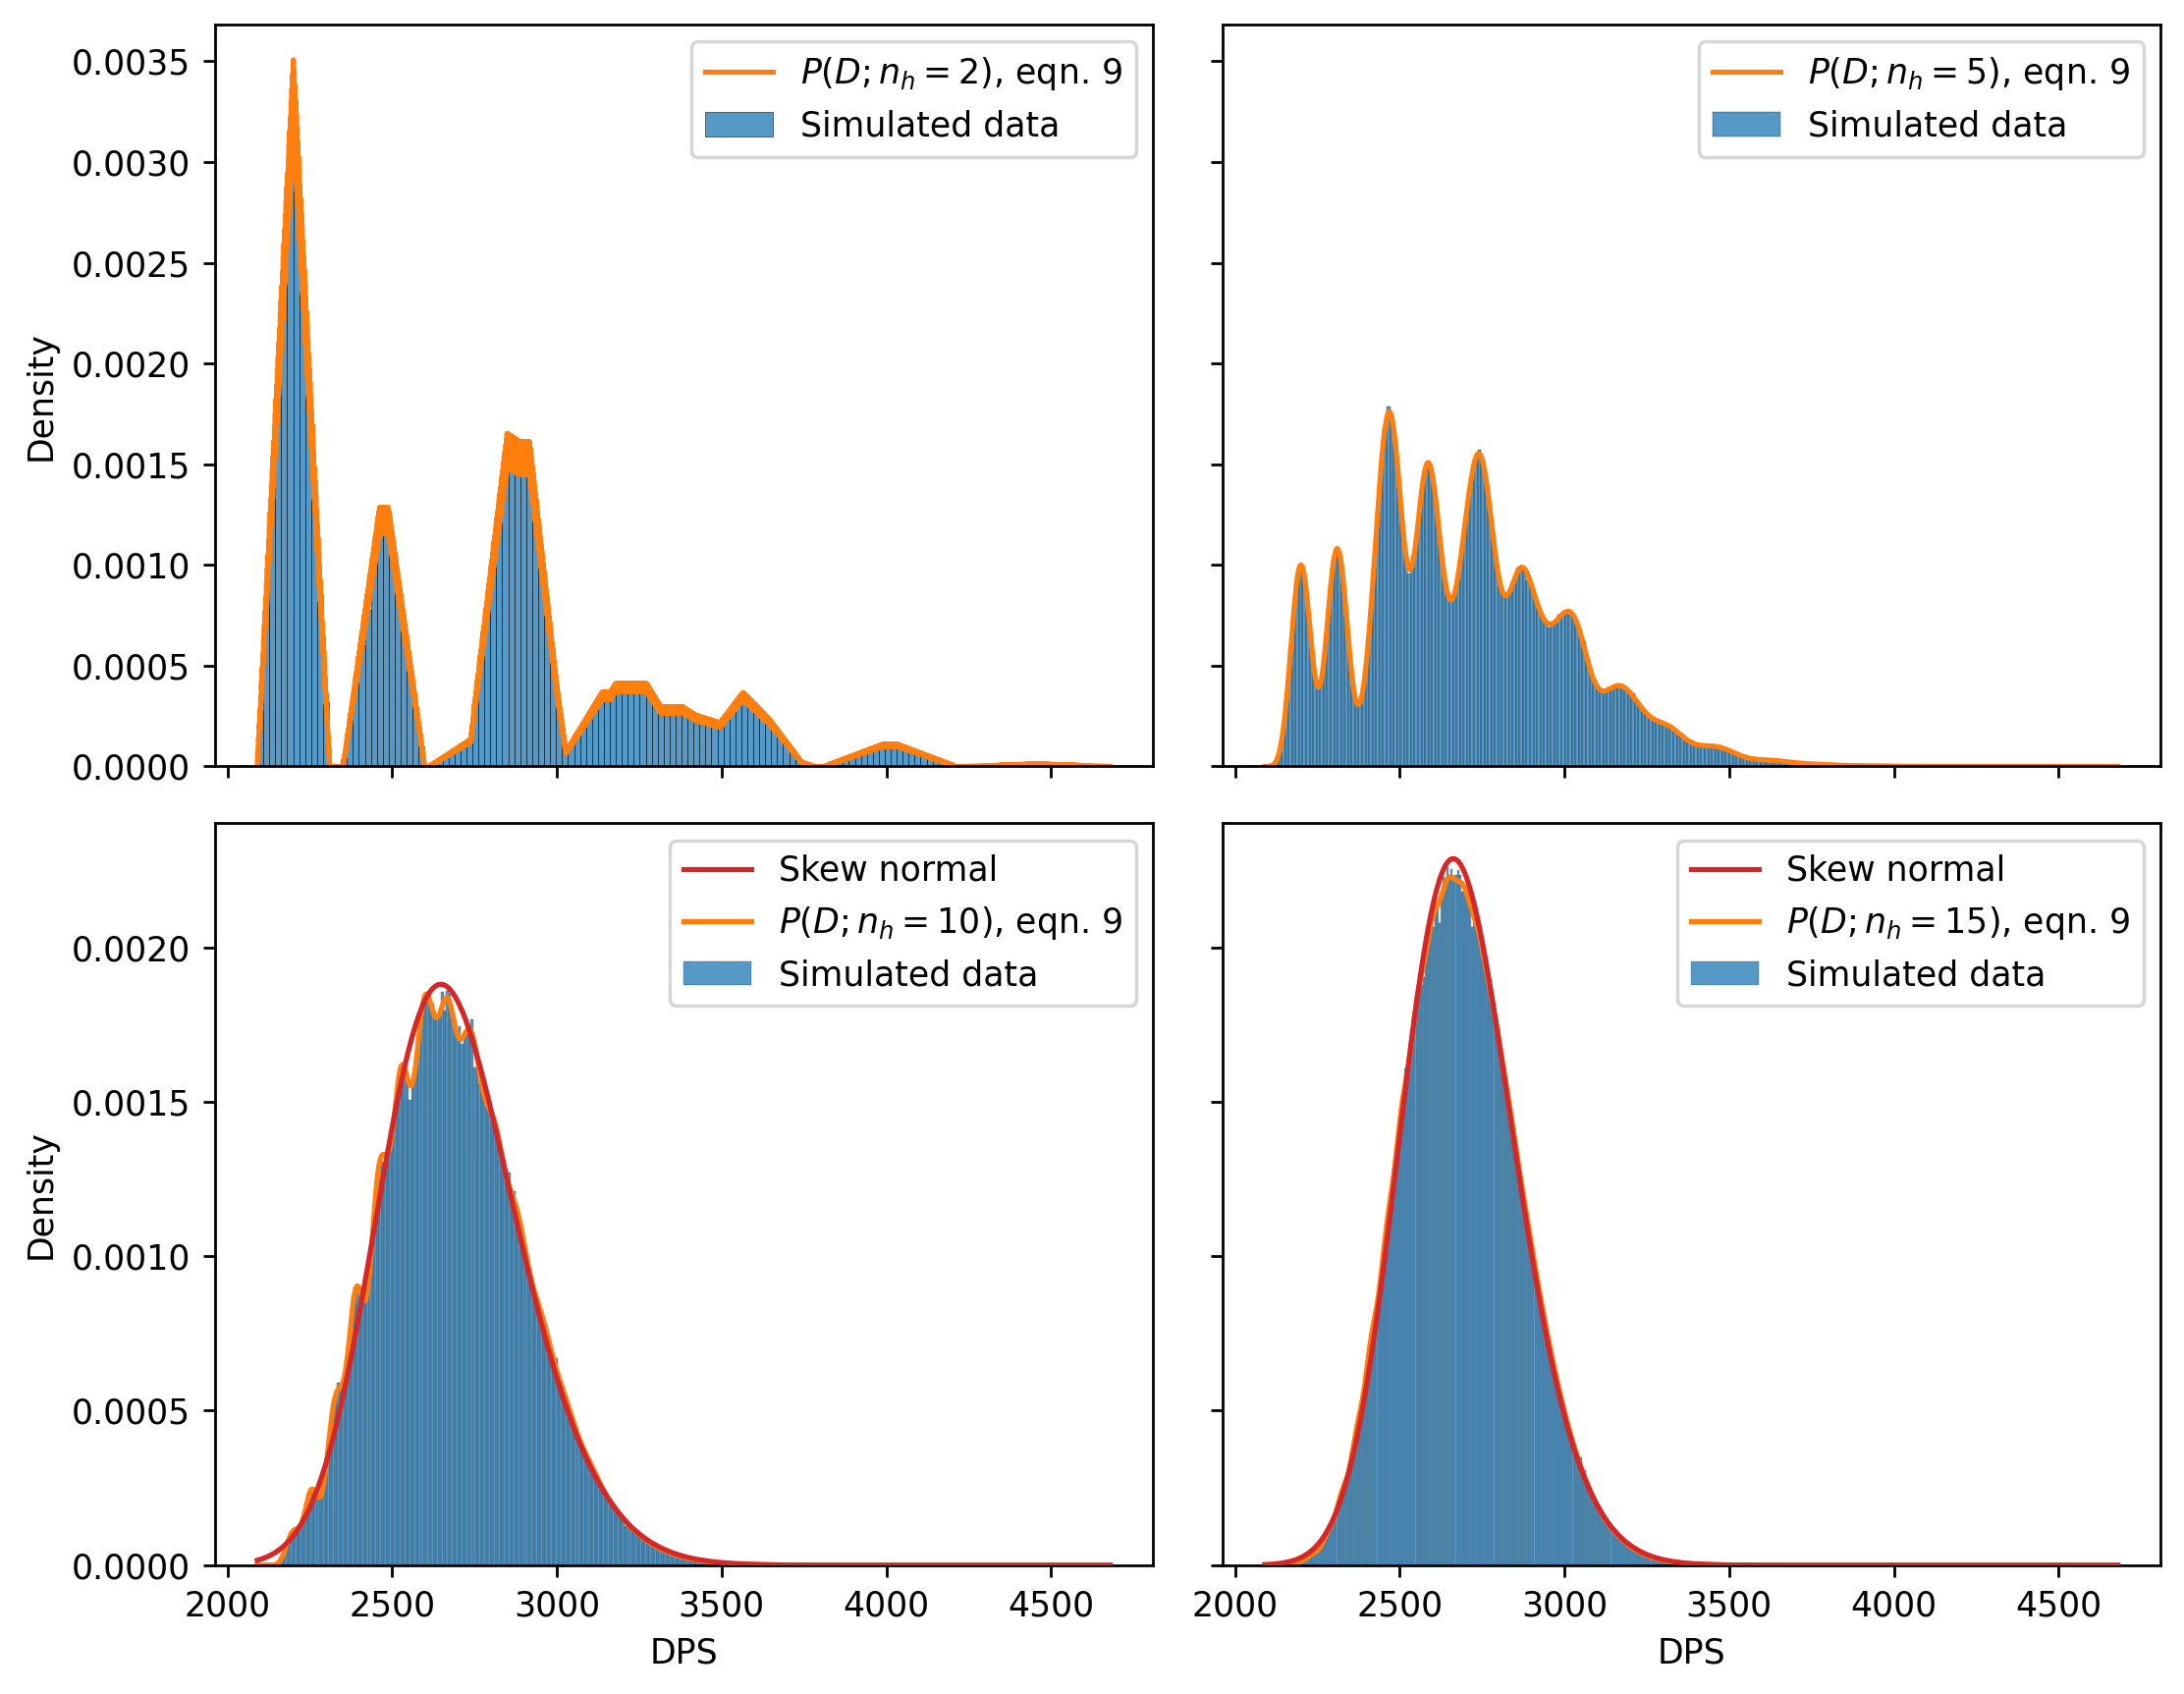
\includegraphics[width=0.95\linewidth]{img/skew-norm-fits.png}
        \caption{DPS distributions from Figure \ref{fig:convo-convergence} plus DPS distributions parameterized to a skew normal distribution for $n_h = 10$ and $n_h = 15$.}\label{fig:skew-norm-fits}
    \end{figure}
    % TODO: mention how this can be combined with deterministic portion to get rotation distribution.
    % https://galaxykate0.tumblr.com/post/139774965871/so-you-want-to-build-a-generator
\end{document}

